%!TEX root = ../larxxia.tex

\section{Subspaces, basis and dimension}
\label{sec:sbd}
\secttoc

\begin{comment}
\pooliv{\S3.5, p191--206} \layiv{\S4.1--3} \holti{\S4.1--3}
\end{comment}


\begin{quoted}{\index{Galileo Galilei}Galileo Galilei, 1610}
%Philosophy is written in this grand book---I mean the universe---which stands continually open to our gaze, but the book cannot be understood unless one first learns to comprehend the language and read the letters in which it is composed.  
%It is written in the language of mathematics.  
%Its characters are triangles, circles and other geometrical figures without which it is humanly impossible to understand a single word of it; without these, one is wandering about in a dark labyrinth.
[Nature] is written in that great book which ever lies before our eyes---I mean the universe---but we cannot understand it if we do not first learn the language and grasp the symbols in which it is written. 
The book is written in the mathematical language, and the symbols are triangles, circles, and other geometric figures, without whose help it is impossible to comprehend a single word of it; without which one wanders in vain through a dark labyrinth.
%(as quoted by Kline, 1972, pp. 328--329. See also Machamer 1998a, pp. 64--65 for a slightly different translation.)
\end{quoted}


Some of the most fundamental geometric structures in mathematics, especially linear algebra, are the lines or planes through the origin, and higher dimensional analogues.
For example, a general solution of linear equations often involve linear combinations such as \((-2,1,0,0)s+(-\frac{15}7,0,\frac97,1)t\) (\autoref{eg:homosysiv}) and \(y_3\vv_3+y_4\vv_4\) (\autoref{eg:3x4findc}): such combinations for all values of the free variables forms a plane through the origin (\autoref{sec:nvep}).
The aim of this section is to connect geometric structures, such as lines and planes, to the information in a singular value decomposition.
The structures are called~\idx{subspace}s.


\subsection{Subspaces are lines, planes, and so on}

\index{subspace|(}
\begin{example} \label{eg:viewsubs}
The following graphs illustrate the concept of subspaces through examples (imagine the graphs extend to infinitely as appropriate).
\begin{enumerate}
\newcommand{\PB}[1]{\quad\parbox[b]{11em}{\raggedright #1}}
\item\label{eg:viewsubsa} 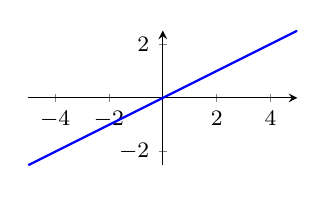
\begin{tikzpicture} 
\begin{axis}[footnotesize,font=\footnotesize
    ,axis equal image, axis lines=middle] 
    \addplot[blue,thick] {x/2};
\end{axis}
\end{tikzpicture}
\PB{is a subspace as it is a straight line through the origin.}

\item 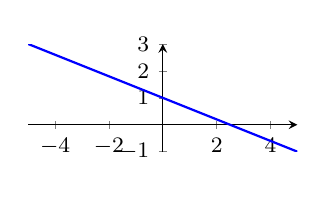
\begin{tikzpicture} 
\begin{axis}[footnotesize,font=\footnotesize
    ,axis equal image, axis lines=middle ] 
    \addplot[blue,thick] {1-0.4*x};
\end{axis}
\end{tikzpicture}
\PB{is \emph{not} a subspace as it does not include the origin.}

\item\label{eg:viewsubsc} 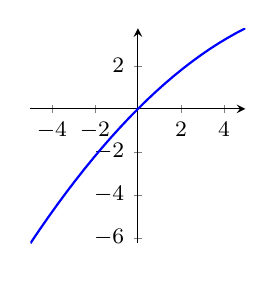
\begin{tikzpicture} 
\begin{axis}[footnotesize,font=\footnotesize
    ,axis equal image, axis lines=middle ] 
    \addplot[blue,thick] {x-x^2/20};
\end{axis}
\end{tikzpicture}
\PB{is \emph{not} a subspace as it curves.}

\item 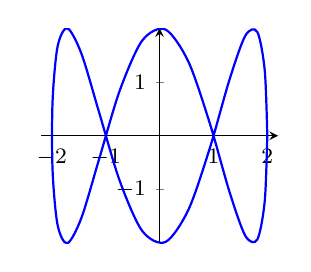
\begin{tikzpicture} 
\begin{axis}[footnotesize,font=\footnotesize,xmin=-2.2,xmax=2.2
    ,axis equal image, axis lines=middle ] 
    \addplot[blue,smooth,samples=30,domain=0:360,thick] ({2*cos(x)},{2*sin(3*x)});
\end{axis}
\end{tikzpicture}
\PB{is \emph{not} a subspace as it not only curves, but does not include the origin.}

\item 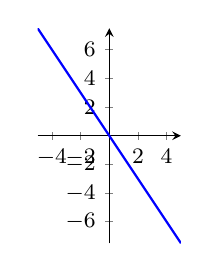
\begin{tikzpicture} 
\begin{axis}[footnotesize,font=\footnotesize
    ,axis equal image, axis lines=middle ] 
    \addplot[blue,thick] {-1.5*x};
\end{axis}
\end{tikzpicture}
\PB{is a subspace.}

\item\label{eg:viewsubsf} 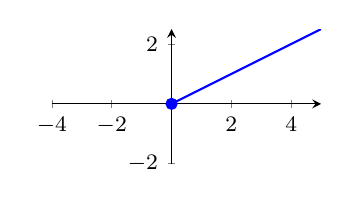
\begin{tikzpicture} 
\begin{axis}[footnotesize,font=\footnotesize,xmin=-4,ymin=-2
    ,axis equal image, axis lines=middle ] 
    \addplot[blue,thick,domain=0:5] {x/2};
    \addplot[only marks,blue] coordinates {(0,0)};
\end{axis}
\end{tikzpicture}
\PB{where the disc indicates an end to the line, is \emph{not} a subspace as it does not extend infinitely in both directions.}

\item 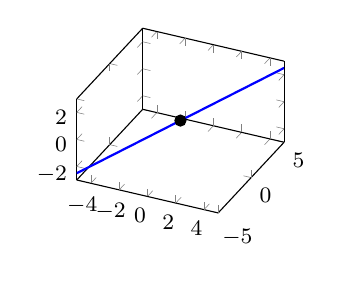
\begin{tikzpicture} 
\begin{axis}[footnotesize,font=\footnotesize
    ,axis equal image    ] 
    \addplot3[blue,samples y=0,thick] ({x},{x},{x/2});
    \addplot3[only marks,black] coordinates {(0,0,0)};
\end{axis}
\end{tikzpicture}
\PB{is a subspace as it is a line through the origin (marked in these 3D plots).}

\item\label{eg:viewsubsh} 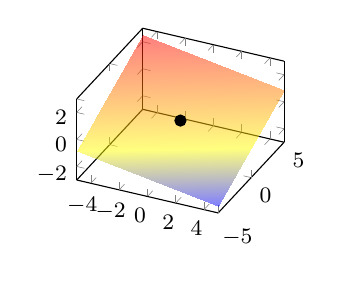
\begin{tikzpicture} 
\begin{axis}[footnotesize,font=\footnotesize
    ,axis equal image    ] 
    \addplot3[surf,shader=interp,samples=2,opacity=0.5] {-x/6+y/3};
    \addplot3[only marks,black] coordinates {(0,0,0)};
\end{axis}
\end{tikzpicture}
\PB{is a subspace as it is a plane through the origin.}

\item\label{eg:viewsubsi} 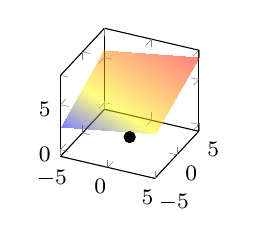
\begin{tikzpicture} 
\begin{axis}[footnotesize,font=\footnotesize
    ,axis equal image    ] 
    \addplot3[only marks,black] coordinates {(0,0,0)};
    \addplot3[surf,shader=interp,samples=2,opacity=0.5] {5+x/6+y/3};
\end{axis}
\end{tikzpicture}
\PB{is \emph{not} a subspace as it does not go through the origin.}

\item 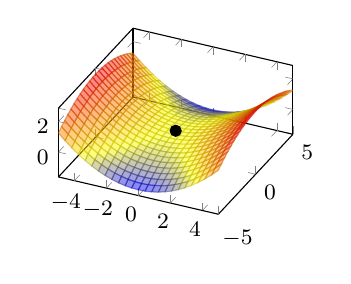
\begin{tikzpicture} 
\begin{axis}[footnotesize,font=\footnotesize
    ,axis equal image, width=13em    ] 
    \addplot3[only marks,black] coordinates {(0,0,0)};
    \addplot3[surf,opacity=0.5] {x^2/10-y^2/20};
\end{axis}
\end{tikzpicture}
\PB{is \emph{not} a subspace as it curves.}

\end{enumerate}
\end{example}



\begin{activity}
Given the examples and comments of \autoref{eg:viewsubs},
which of the following is a subspace?
\actposs{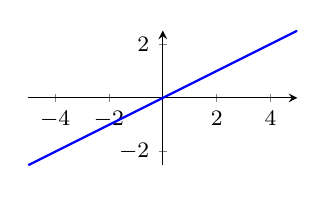
\begin{tikzpicture} 
\begin{axis}[footnotesize,font=\footnotesize
    ,axis equal image, axis lines=middle ] 
    \addplot[blue,thick] {x/2};
\end{axis} \end{tikzpicture}}
{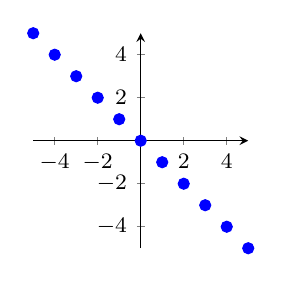
\begin{tikzpicture} 
\begin{axis}[footnotesize,font=\footnotesize
    ,axis equal image, axis lines=middle ] 
    \addplot[blue,only marks,samples=11] {-x};
\end{axis} \end{tikzpicture}}
{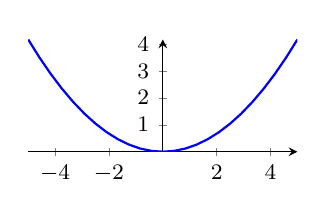
\begin{tikzpicture} 
\begin{axis}[footnotesize,font=\footnotesize
    ,axis equal image, axis lines=middle ] 
    \addplot[blue,thick] {x^2/6};
\end{axis} \end{tikzpicture}}
{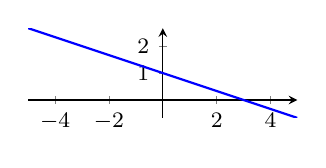
\begin{tikzpicture} 
\begin{axis}[footnotesize,font=\footnotesize
    ,axis equal image, axis lines=middle ] 
    \addplot[blue,thick] {1-x/3};
\end{axis} \end{tikzpicture}}
%\begin{parts}
%\item \begin{tikzpicture} 
%\begin{axis}[footnotesize,font=\footnotesize
%    ,axis equal image, axis lines=middle ] 
%    \addplot[blue,only marks,samples=11] {-x};
%\end{axis} \end{tikzpicture}
%\item \begin{tikzpicture} 
%\begin{axis}[footnotesize,font=\footnotesize
%    ,axis equal image, axis lines=middle ] 
%    \addplot[blue,thick] {x^2/6};
%\end{axis} \end{tikzpicture}
%\item \begin{tikzpicture} 
%\begin{axis}[footnotesize,font=\footnotesize
%    ,axis equal image, axis lines=middle ] 
%    \addplot[blue,thick] {x/2};
%\end{axis} \end{tikzpicture}
%\item \begin{tikzpicture} 
%\begin{axis}[footnotesize,font=\footnotesize
%    ,axis equal image, axis lines=middle ] 
%    \addplot[blue,thick] {1-x/3};
%\end{axis} \end{tikzpicture}
%\end{parts}
\end{activity}




The following definition expresses precisely in algebra the concept of a subspace.
This book uses the `blackboard bold' font, such as \WW\ and~\RR, for names of spaces and subspaces.

% I think we need to use \in by now, if not already invoked
Recall that the mathematical symbol~``\(\in\)''\index{in, $\in$}\index{$\in$} means~``in'' or ``in the set'' or ``is an element of the set''.
For two examples: ``\(c\in\RR\)'' means ``\(c\)~is a real number''; whereas ``\(\vv\in\RR^3\)'' means ``\(\vv\)~is a vector with three components.
Hereafter, this book uses~``\(\in\)'' extensively.


\begin{definition} \label{def:subspace} 
A \bfidx{subspace}~\WW\ of~\(\RR^n\),  is a set of vectors with \(\ov\in\WW\) and such that \WW\ is \idx{closed} under addition and scalar multiplication: that is, for all \(c\in\RR\) and for all \(\uv,\vv\in\WW\), then both \(\uv+\vv\in\WW\) and \(c\uv\in\WW\).
\end{definition}


\begin{example} \label{eg:somsubs}
Use \autoref{def:subspace} to show why each of the following are subspaces, or not. 
\begin{enumerate}
\item All vectors in the line \(y=x/2\) (\autoref{eg:viewsubsa}).
\begin{solution} 
The origin~\ov\ is in the line \(y=x/2\) as \(x=y=0\) satifies the equation.
\marginpar{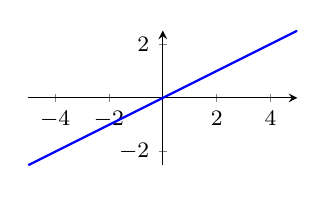
\begin{tikzpicture} 
\begin{axis}[footnotesize,font=\footnotesize
    ,axis equal image, axis lines=middle] 
    \addplot[blue,thick] {x/2};
\end{axis}
\end{tikzpicture}}%
The line \(y=x/2\) is composed of vectors in the form \(\uv=(1,\frac12)t\) for some parameter~\(t\).
Then for any \(c\in\RR\)\,, \(c\uv=c(1,\frac12)t=(1,\frac12)(ct)=(1,\frac12)t'\) for new parameter \(t'=ct\)\,; hence \(c\uv\)~is in the line.
Let \(\vv=(1,\frac12)s\) be another vector in the line for some parameter~\(s\), then \(\uv+\vv=(1,\frac12)t+(1,\frac12)s=(1,\frac12)(t+s)=(1,\frac12)t'\) for new parameter \(t'=t+s\)\,; hence \(\uv+\vv\) is in the line.
The three requirements of \autoref{def:subspace} are met, and so this line is a subspace. 
\end{solution}

\item All vectors \((x,y)\) such that \(y=x-x^2/20\) (\autoref{eg:viewsubsc}).
\begin{solution} 
A vector is `in the set' when its end-point lies on a plot of the set, as in the margin.
\marginpar{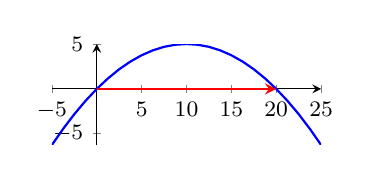
\begin{tikzpicture} 
\begin{axis}[footnotesize,font=\footnotesize,domain=-5:25
    ,axis equal image, axis lines=middle ] 
    \addplot[blue,thick] {x-x^2/20};
    \addplot[red,thick,quiver={u=20,v=0},-stealth] coordinates {(0,0)};
\end{axis}
\end{tikzpicture}}%
To show something is not a subspace, we only need to give one instance when one of the properties fail.
One instance is that the vector \((20,0)\) is in the curve as \(20-20^2/20=0\)\,, but the scalar multiple of half of this vector \(\frac12(20,0)=(10,0)\) is not as \(10-10^2/20=5\neq0\)\,.
That is, the curve is not closed under scalar multiplication and hence is not a subspace. 
\end{solution}

\item All vectors \((x,y)\) in the line \(y=x/2\) for \(x,y\geq0\) (\autoref{eg:viewsubsf}).
\begin{solution} 
A vector is `in the set' when its end-point lies on a plot of the set, as in the margin.
\marginpar{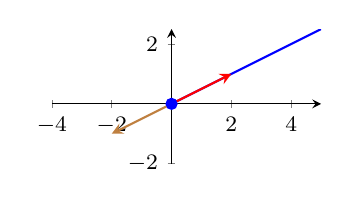
\begin{tikzpicture} 
\begin{axis}[footnotesize,font=\footnotesize,xmin=-4,ymin=-2
    ,axis equal image, axis lines=middle ] 
    \addplot[blue,thick,domain=0:5] {x/2};
    \addplot[only marks,blue] coordinates {(0,0)};
    \addplot[red,thick,quiver={u=2,v=1},-stealth] coordinates {(0,0)};
    \addplot[brown,thick,quiver={u=-2,v=-1},-stealth] coordinates {(0,0)};
\end{axis}
\end{tikzpicture}}%
Although vectors \((x,y)\) in the line \(y=x/2\) for \(x,y\geq0\) includes the origin and is closed under addition, it fails the scalar multiplication test.
For example, \(\uv=(2,1)\) is in the line, but the scalar multiple \((-1)\uv=(-2,-1)\) is not.
Hence it is not a subspace.
\end{solution}


\item All vectors \((x,y,z)\) in the plane \(z=-x/6+y/3\) (\autoref{eg:viewsubsh}).
\begin{center}
\qview{30}{34}{\begin{tikzpicture} 
\begin{axis}[footnotesize,font=\footnotesize
    ,axis equal image ,view={\q}{30}   ] 
    \addplot3[surf,shader=interp,samples=2,opacity=0.5] {-x/6+y/3};
    \addplot3[only marks,black] coordinates {(0,0,0)};
\end{axis}
\end{tikzpicture}}
\end{center}
\begin{solution} 
The origin~\ov\ is in the plane \(z=-x/6+y/3\) as \(x=y=z=0\) satisfies the equation.
A vector \(\uv=(u_1,u_2,u_3)\) is in the plane provided \(-u_1+2u_2-6u_3=0\)\,.
Consider \(c\uv=(cu_1,cu_2,cu_3)\) for which \(-(cu_1)+2(cu_2)-6(cu_3) =c(-u_1+2u_2-6u_3) =c\times0=0\) and hence must also be in the plane.
Also let vector \(\vv=(v_1,v_2,v_3)\) be in the plane and consider \(\uv+\vv=(u_1+v_1,u_2+v_2,u_3+v_3)\) for which \(-(u_1+v_1)+2(u_2+v_2)-6(u_3+v_3) =-u_1-v_1+2u_2+2v_2-6u_3-6v_3 =(-u_1+2u_2-6u_3) +(-v_1+2v_2-6v_3) =0+0 =0\) and hence must also be in the plane.
The three requirements of \autoref{def:subspace} are met, and so this plane is a subspace.
\end{solution}


\item All vectors \((x,y,z)\) in the plane \(z=5+x/6+y/3\) (\autoref{eg:viewsubsi}).
\begin{center}
\qview{30}{34}{\begin{tikzpicture} 
\begin{axis}[small,font=\footnotesize
    ,axis equal image  ,view={\q}{30}  ] 
    \addplot3[only marks,black] coordinates {(0,0,0)};
    \addplot3[red,thick,quiver={u=0,v=0,w=5},-stealth] coordinates {(0,0,0)};
    \addplot3[surf,shader=interp,samples=2,opacity=0.5] {5+x/6+y/3};
\end{axis}
\end{tikzpicture}}
\end{center}
\begin{solution} 
In this case, consider the vector \(\uv=(0,0,5)\) (shown in the above picture): any scalar multiple, say \(2\uv=(0,0,10)\), is not in the plane.
That is, vectors in the plane are not closed under scalar multiplication, and hence the plane is not a subspace.
\end{solution}


\item\label{eg:somsubsf} \(\{\ov\}\).
\begin{solution} 
The zero vector forms a trivial subspace, \(\WW=\{\ov\}\)\,:  firstly, \(\ov\in\WW\);
secondly, the only vector in~\WW\ is \(\uv=\ov\) for which every scalar multiple \(c\uv=c\ov=\ov\in\WW\);
and thirdly, a second vector~\vv\ in~\WW\ can only be \(\vv=\ov\) so \(\uv+\vv=\ov+\ov=\ov\in\WW\).
The three requirements of \autoref{def:subspace} are met, and so \(\{\ov\}\) is always a subspace. 
\end{solution}

\item\label{eg:somsubsg} \(\RR^n\).
\begin{solution} \sloppy
Lastly, \(\RR^n\) also is a subspace:
firstly, \(\ov=(0,0,\ldots,0)\in\RR^n\);
secondly, for \(\uv=(\hlist un)\in\RR^n\), the scalar multiplication \(c\uv=c(\hlist un) =(\hlist{cu}n)\in\RR^n\);
and thirdly, for \(\vv=(\hlist vn)\in\RR^n\), the vector addition \(\uv+\vv=(\hlist un)+(\hlist vn) =(u_1+v_1,u_2+v_2,\ldots,u_n+v_n)\in\RR^n\).
The three requirements of \autoref{def:subspace} are met, and so \(\RR^n\) is always a subspace. 
\end{solution}

\end{enumerate}
\end{example}



\begin{activity}
The following pairs of vectors are all in the set shown in the margin (in the sense that their end-points lie on the plotted curve).  
\marginpar{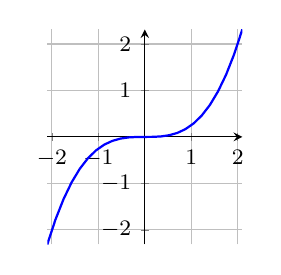
\begin{tikzpicture} 
\begin{axis}[footnotesize,font=\footnotesize
    ,axis equal image, axis lines=middle, grid ] 
    \addplot[blue,thick,domain=-2.1:2.1] {x^3/4};
\end{axis} \end{tikzpicture}}%
The sum of which pair proves that the curve plotted in the margin is not a subspace?
\actposs{\((-1,-\frac14),\ (2,2)\)}
{\((0,0),\ (2,2)\)}
{\((2,2),\ (-2,-2)\)}
{\((1,\frac14),\ (0,0)\)}
%\begin{parts}
%\item \((0,0),\ (2,2)\)
%\item \((2,2),\ (-2,-2)\)
%\item \((1,\frac14),\ (0,0)\)
%\item \((-1,-\frac14),\ (2,2)\)
%\end{parts}
\end{activity}




In summary:
\begin{itemize}
\item in two dimensions~(\(\RR^2\)), subspaces are the origin~\ov, a line through~\ov, or the entire plane~\(\RR^2\);
\item in three dimensions~(\(\RR^3\)), subspaces are the origin~\ov, a line through~\ov, a plane through~\ov, or the entire space~\(\RR^3\);
\item and analogously for higher dimensions~(\(\RR^n\)).
\end{itemize}


Recall that the set of all linear combinations of a set of vectors, such as \((-2,1,0,0)s+(-\frac{15}7,0,\frac97,1)t\) (\autoref{eg:homosysiv}), is called the span of that set (\autoref{def:span}).

\begin{theorem} \label{thm:spansubs} 
Let \hlist\vv k\ be \(k\)~vectors in~\(\RR^n\),
then \(\Span\{\hlist\vv k\}\) is a \idx{subspace} of~\(\RR^n\).
\end{theorem}

\begin{proof}
Denote \(\Span\{\hlist\vv k\}\) by~\WW; we aim to prove it is a subspace (\autoref{def:subspace}).
First, \(\ov=0\vv_1+0\vv_2+\cdots+0\vv_k\) which is a linear combination of \hlist\vv k\,, and so the zero vector \(\ov\in\WW\).
Now let \(\uv,\vv\in\WW\) then by \autoref{def:span} there are coefficients \hlist an\ and \hlist bn\ such that
\begin{eqnarray*}
&&\uv=\lincomb a\vv k\,,
\\&&\vv=\lincomb b\vv k\,.
\end{eqnarray*}
Secondly, consequently
\begin{eqnarray*}
\uv+\vv&=&
\lincomb a\vv k
\\&&{}+\lincomb b\vv k
\\&=&(a_1+b_1)\vv_1+(a_2+b_2)\vv_2+\cdots+(a_k+b_k)\vv_k\,,
%\\&\in&\Span\{\hlist\vv k\}=\WW.
\end{eqnarray*}
which is a linear combination of \hlist\vv k\,, and so is in~\WW.
Thirdly, for any scalar~\(c\),
\begin{eqnarray*}
c\uv&=&c(\lincomb a\vv k)
\\&=&\lincomb {ca}\vv k\,,
%\\&\in&\Span\{\hlist\vv k\}=\WW.
\end{eqnarray*}
which is a linear combination of \hlist\vv k\,, and so is in~\WW.
Hence \(\WW=\Span\{\hlist\vv k\}\) is a subspace.
\end{proof}


\begin{example} \label{eg:1x2subs}
\(\Span\{(1,\frac12)\}\) is the subspace \(y=x/2\).
The reason is that a vector \(\uv\in\Span\{(1,\frac12)\}\) only if there is some constant~\(a_1\) such that \(\uv=a_1(1,\frac12)=(a_1,a_1/2)\).
That is, the \(y\)-component is half the \(x\)-component and hence it lies on the line \(y=x/2\).

\(\Span\{(1,\frac12),(-2,-1)\}\) is also the subspace \(y=x/2\) since every linear combination \(a_1(1,\frac12)+a_2(-2,-1)=(a_1-2a_2,a_1/2-a_2)\) satisfies that the \(y\)-component is half the \(x\)-component and hence the linear combination lies on the line \(y=x/2\).
\end{example}


\begin{example} \label{eg:plsubs}
The plane \(z=-x/6+y/3\) may be written as \(\Span\{(3,3,1/2),(0,3,1)\}\), as illustrated in stereo below, since every linear combination of these two vectors fills out the plane: \(a_1(3,3,1/2)+a_2(0,3,1) =(3a_1,3a_1+3a_2,a_1/2+a_2)\) and so lies in the plane as \(-x/6+y/3-z=-\frac163a_1+\frac13(3a_1+3a_2)-(a_1/2+a_2) =-\frac12a_1+a_1+a_2-\frac12a_1-a_2=0\) for all \(a_1\) and~\(a_2\) (although such arguments do not establish that the linear combinations cover the whole plane---we need \autoref{thm:homosubsp}).
\begin{center}
\qview{28}{32} {\begin{tikzpicture} 
\begin{axis}[footnotesize,font=\footnotesize
    ,axis equal image  ,view={\q}{30}  ] 
    \addplot3[surf,shader=interp,samples=2,blue,opacity=0.4] {-x/6+y/3};
    \addplot3[blue!50!black,thick,quiver={u=3,v=3,w=1/2},-stealth] coordinates {(0,0,0)};
    \addplot3[blue!50!black,thick,quiver={u=0,v=3,w=1},-stealth] coordinates {(0,0,0)};
\end{axis}
\end{tikzpicture}}
\end{center}

Also,  \(\Span\{(5,1,-1/2),(0,-3,-1),(-4,1,1)\}\) is the  plane \(z=-x/6+y/3\), as illustrated below. 
The reason is that every linear combination of these three vectors fills out the plane: \(a_1(5,1,-1/2)+a_2(0,-3,-1)+a_3(-4,1,1) =(5a_1-4a_3, a_1-3a_2+a_3, -a_1/2-a_2+a_3)\) and so lies in the plane as \(-x/6+y/3-z=-\frac16(5a_1-4a_3)+\frac13(a_1-3a_2+a_3)-(-a_1/2-a_2+a_3) =-\frac56a_1+\frac23a_3+\frac13a_1-a_2+\frac13a_3+\frac12a_1+a_2-a_3 =0\) for all \(a_1\), \(a_2\) and~\(a_3\).
\begin{center}
\qview{28}{32} {\begin{tikzpicture} 
\begin{axis}[small,font=\footnotesize
    ,axis equal image  ,view={\q}{35}  ] 
    \addplot3[surf,shader=interp,samples=2,blue,opacity=0.4] {-x/6+y/3};
    \addplot3[blue!50!black,thick,quiver={u=5,v=1,w=-1/2},-stealth] coordinates {(0,0,0)};
    \addplot3[blue!50!black,thick,quiver={u=0,v=-3,w=-1},-stealth] coordinates {(0,0,0)};
    \addplot3[blue!50!black,thick,quiver={u=-4,v=1,w=1},-stealth] coordinates {(0,0,0)};
\end{axis}
\end{tikzpicture}}
\end{center}
\end{example}

\begin{example} \label{eg:planesubs}
Find a set of two vectors that spans the plane \(x-2y+3z=0\)\,.
\begin{solution} 
Write the equation for this plane as \(x=2y-3z\)\,, say, then vectors in the plane are all of the form \(\uv=(x,y,z)=(2y-3z,y,z) =(2,1,0)y+(-3,0,1)z\)\,.
That is, all vectors in the plane may be written as a linear combination of the two vectors \((2,1,0)\) and~\((-3,0,1)\),
hence the plane is \(\Span\{(2,1,0),(-3,0,1)\}\) as illustrated in stereo below. 
\begin{center}
\qview{28}{32} {\begin{tikzpicture} 
\begin{axis}[small,font=\footnotesize,domain=-3:3
    ,axis equal image  ,view={\q}{30}  ] 
    \addplot3[surf,shader=interp,samples=2,blue,opacity=0.4] {-x/3+y*2/3};
    \addplot3[blue!50!black,thick,quiver={u=+2,v=1,w=0},-stealth] coordinates {(0,0,0)};
    \addplot3[blue!50!black,thick,quiver={u=-3,v=0,w=1},-stealth] coordinates {(0,0,0)};
\end{axis}
\end{tikzpicture}}
\end{center}
\end{solution}
\end{example}



Such subspaces connect with matrices.
The connection is via a matrix whose columns are the vectors appearing within the span.
Although sometimes we also use the rows of the matrix to be the vectors in the span.


\begin{definition}\label{def:colsp} 
    \begin{enumerate}
        \item\label{def:colspa} The \bfidx{column space} of any $m\times n$ matrix~$A$ is the \idx{subspace} of~$\RR^m$ \idx{span}ned by the \(n\)~\idx{column vector}s of~$A$.
        \footnote{Some of you will know that the column space is also called the \idx{range}, but for the moment we just use the term column space. \ifcsname r@ch:cipvs\endcsname \autoref{ch:cipvs} establishes and discusses this connection between column space and range.\fi}
        
		\item\label{def:colspb} The \bfidx{row space} of any $m\times n$ matrix~$A$ is the \idx{subspace} of~$\RR^n$ \idx{span}ned by the \(m\)~\idx{row vector}s of~$A$.  
    \end{enumerate}
\end{definition}


\begin{example} \label{eg:}
Examples~\ref{eg:1x2subs}--\ref{eg:planesubs} provide some cases.
\begin{itemize}
\item From \autoref{eg:1x2subs}, the column space of \(A=\footnotesize\begin{bmatrix} 1&-2\\\frac12&-1 \end{bmatrix}\) is the line \(y=x/2\)\,.

The row space of this matrix~\(A\) is \(\Span\{(1,-2),(\frac12,-1)\}\).
\marginpar{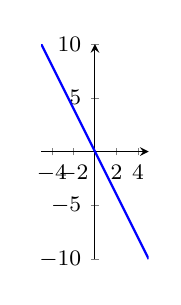
\begin{tikzpicture} 
\begin{axis}[footnotesize,font=\footnotesize
    ,axis equal image, axis lines=middle] 
    \addplot[blue,thick] {-2*x};
\end{axis}
\end{tikzpicture}}%
This row space is the set of all vectors of the form \((1,-2)s+(\frac12,-1)t=(s+t/2,-2s-t)=(1,-2)(s+t/2)=(1,-2)t'\) is the line \(y=-2x\) as illustrated in the margin.
That the row space and the column space are both lines, albeit different lines, is not a coincidence (\autoref{thm:rowcolD}).

\item \autoref{eg:plsubs} shows that the column space of matrix
\begin{equation*}
B=\begin{bmatrix} 3&0\\3&3\\\frac12&1 \end{bmatrix}
\end{equation*}
is the plane \(z=-x/6+y/3\) in~\(\RR^3\).

The row space of matrix~\(B\) is \(\Span\{(3,0),(3,3),(\frac12,1)\}\) which is a subspace of~\(\RR^2\), whereas the column space is a subspace of~\(\RR^3\).
\marginpar{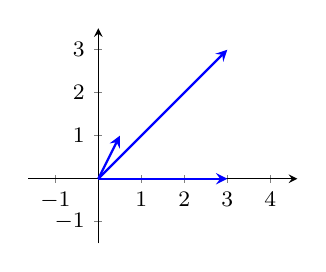
\begin{tikzpicture} 
\begin{axis}[footnotesize,font=\footnotesize,ymin=-1.5,ymax=3.5
    ,axis equal, axis lines=middle ] 
    \addplot[blue,thick,quiver={u=3,v=0},-stealth] coordinates {(0,0)};
    \addplot[blue,thick,quiver={u=3,v=3},-stealth] coordinates {(0,0)};
    \addplot[blue,thick,quiver={u=1/2,v=1},-stealth] coordinates {(0,0)};
\end{axis}
\end{tikzpicture}}%
Here the span is all of~\(\RR^2\) as for each \((x,y)\in\RR^2\) choose  the linear combination \(\frac{x-y}3(3,0)+\frac{y}3(3,3)+0(\frac12,1)=(x-y+y+0,0+y+0)=(x,y)\) so each \((x,y)\) is in the span, and hence all of the \(\RR^2\)~plane is the span.
That the column space and the row space are both planes is no coincidence (\autoref{thm:rowcolD}).

\item \autoref{eg:plsubs} also shows that the column space of matrix
\begin{equation*}
C=\begin{bmatrix} 5&0&-4\\1&-3&1\\-\frac12&-1&1 \end{bmatrix}
\end{equation*}
is also the plane \(z=-x/6+y/3\) in~\(\RR^3\).

Now, \(\Span\{(5,0,-4),(1,-3,1),(-\frac12,-1,1)\}\) is the row space of matrix~\(C\).
It is not readily apparent but we can check that this space is the plane \(4x+3y+5z=0\) as illustrated below in stereo.
To see this, consider all linear combinations \(a_1(5,0,-4)+a_2(1,-3,1)+a_3(-\frac12,-1,1)
=(5a_1+a_2-a_3/2, -3a_2-a_3, -4a_1+a_2+a_3)\) satisfy
\(4x+3y+5z
=4(5a_1+a_2-a_3/2)+3(-3a_2-a_3)+5(-4a_1+a_2+a_3)
=20a_1+4a_2-2a_3-9a_2-3a_3-20a_1+5a_2+5a_3
=0\)\,.
\begin{center}
\qview{73}{75}{\begin{tikzpicture} 
\begin{axis}[small,font=\footnotesize,view={\q}{30}
    ,axis equal image    ] 
    \addplot3[surf,shader=interp,samples=2,blue,opacity=0.4] {-0.8*x-0.6*y};
    \addplot3[blue!50!black,thick,quiver={u=5,v=0,w=-4},-stealth] coordinates {(0,0,0)};
    \addplot3[blue!50!black,thick,quiver={u=1,v=-3,w=1},-stealth] coordinates {(0,0,0)};
    \addplot3[blue!50!black,thick,quiver={u=-1/2,v=-1,w=1},-stealth] coordinates {(0,0,0)};
\end{axis}
\end{tikzpicture}}%
\end{center}
Again, it is no coincidence that the row and column spaces of~\(C\) are both planes (\autoref{thm:rowcolD}).
\end{itemize}
\end{example}





\begin{activity}
Which one of the following vectors is in the column space of the matrix
\begin{equation*}
\begin{bmatrix} 6 &  2
\\  -3 &  5
\\  -2 & -1 \end{bmatrix}?
\end{equation*}
\actposs[4]{\(\begin{bmatrix} 8\\2\\-3 \end{bmatrix}\)}
{\(\begin{bmatrix} 2\\-3\\-3 \end{bmatrix}\)}
{\(\begin{bmatrix} 2\\2\\-3 \end{bmatrix}\)}
{\(\begin{bmatrix} 8\\5\\-2 \end{bmatrix}\)}
%\partswidth=5em
%\begin{parts}
%\item \(\begin{bmatrix} 2\\-3\\-3 \end{bmatrix}\)
%\item \(\begin{bmatrix} 2\\2\\-3 \end{bmatrix}\)
%\item \(\begin{bmatrix} 8\\2\\-3 \end{bmatrix}\)
%\item \(\begin{bmatrix} 8\\5\\-2 \end{bmatrix}\)
%\end{parts}
\end{activity}




\begin{example} \label{eg:}
Is vector \(\bv=(-0.6,0,-2.1,1.9,1.2)\) in the \idx{column space} of matrix
\begin{equation*}
A=\begin{bmatrix} 2.8&-3.1&3.4
\\4.0&1.7&0.8
\\-0.4&-0.1&4.4
\\1.0&-0.4&-4.7
\\-0.3&1.9&0.7 \end{bmatrix}?
\end{equation*}
What about vector \(\cv=(15.2,5.4,3.8,-1.9,-3.7)\)?

\begin{solution} 
The question is: can we find a linear combination of the columns of~\(A\) which equals vector~\bv?
That is, can we find some vector~\xv\ such that \(A\xv=\bv\)?
Answer using our knowledge of linear equations.

Let's use \autoref{pro:gensol} in \script.
\begin{enumerate}
\item Compute an \svd\  of this \(5\times 3\) matrix with
\begin{verbatim}
A=[2.8 -3.1  3.4
   4.0  1.7  0.8
  -0.4 -0.1  4.4
   1.0 -0.4 -4.7
  -0.3  1.9  0.7]
[U,S,V]=svd(A)
\end{verbatim}
\setbox\ajrqrbox\hbox{\qrcode{% column space
A=[2.8 -3.1 3.4
 4.0 1.7 0.8
 -0.4 -0.1 4.4
 1.0 -0.4 -4.7
 -0.3 1.9 0.7]
[U,S,V]=svd(A)
z=U'*[-0.6;0;-2.1;1.9;1.2]
z=U'*[15.2;5.4;3.8;-1.9;-3.7]
}}%
\marginpar{\usebox{\ajrqrbox\\[2ex]}}%
to find \twodp
\begin{verbatim}
U =
  -0.58   0.49   0.53  -0.07   0.37
  -0.17   0.69  -0.65  -0.04  -0.25
  -0.56  -0.28  -0.10   0.74  -0.22
   0.57   0.43   0.21   0.66   0.14
  -0.04  -0.15  -0.49   0.10   0.85
S =
   7.52      0      0
      0   4.91      0
      0      0   3.86
      0      0      0
      0      0      0
V = ...
\end{verbatim}

\item Then solve \(U\zv=\bv\) with \verb|z=U'*[-0.6;0;-2.1;1.9;1.2]| to find \twodp\ \(\zv=(2.55,0.92,-0.29,-0.15,1.54)\).

\item Now the diagonal matrix~\(S\) has three non-zero singular values, and the last two rows are zero.
So to be able to solve \(S\yv=\zv\) we need the last two components of~\zv\ to be zero. 
But, at \(-0.15\) and~\(1.54\), they are not zero, so the system is not solvable.
Hence there is no linear combination of the columns of~\(A\) that gives us vector~\bv.
Consequently, vector~\bv\ is not in the column space of~\(A\).

\item For the case of vector~\(\cv=(15.2,5.4,3.8,-1.9,-3.7)\) solve \(U\zv=\cv\) with 
\begin{verbatim}
z=U'*[15.2;5.4;3.8;-1.9;-3.7]
\end{verbatim}
to find \(\zv=(-12.800,9.876,5.533,0.000,0.000)\).
Since the last two entries in vector~\zv\ are zero, corresponding to the zero rows of~\(S\), a solution exists to \(S\yv=\zv\)\,.
Hence a solution exists to \(A\xv=\cv\)\,.
Consequently, vector~\cv\ is in the column space of~\(A\).

\end{enumerate}
(Incidentally, you may check that \(\cv=2\av_1-2\av_2+\av_3\)\,.)
\end{solution}
\end{example}






Another subspace associated with matrices is the set of possible solutions to a homogeneous system of linear equations.


\begin{theorem}\label{thm:homosubsp} 
For any $m\times n$ matrix~$A$, define the set~$\Null(A)$ to be all the solutions~$\xv$ of the \idx{homogeneous} system $A\xv=\ov$\,. 
The set~\(\Null(A)\) is a \idx{subspace} of~$\RR^n$ called the \bfidx{nullspace} of~$A$.
\end{theorem}
\begin{proof} 
First, \(A\ov=\ov\) so \(\ov\in\Null A\)\,.
Let \(\uv,\vv\in\Null A\)\,; that is, \(A\uv=\ov\) and \(A\vv=\ov\)\,.
Second, by the distributivity of matrix-vector multiplication (\autoref{thm:pmm}), \(A(\uv+\vv)=A\uv+A\vv=\ov+\ov=\ov\) and so \(\uv+\vv\in\Null A\)\,.
Third, by the associativity and commutativity of \emph{scalar} multiplication (\autoref{thm:pasm}), for every \(c\in\RR\)\,, \(A(c\uv)=Ac\uv=cA\uv=c(A\uv)=c\ov=\ov\) and so \(c\uv\in\Null A\). 
Hence \(\Null A\) is a subspace (\autoref{def:subspace}).
\end{proof}




\begin{example} \label{eg:nullsp}
\begin{itemize}
\item  \autoref{eg:homosysi} showed that the only solution of the homogeneous system \(\footnotesize\begin{cases}
3x_1-3x_2=0\\-x_1-7x_2=0
\end{cases}\) is \(\xv=\ov\)\,.
Thus its set of solutions is~\(\{\ov\}\) which is a subspace (\autoref{eg:somsubsf}).
Thus \(\{\ov\}\) is the nullspace of matrix \(\footnotesize\begin{bmatrix} 3&-3\\-1&-7 \end{bmatrix}\).

\item Recall the homogeneous system of linear equations from \autoref{eg:homosysiv} has solutions \(\xv=(-2s-\frac{15}7t,s,\frac97t,t) =(-2,1,0,0)s+(-\frac{15}7,0,\frac97,1)t\) for arbitrary \(s\) and~\(t\).
That is, the set of solutions is \(\Span\{(-2,1,0,0),(-\frac{15}7,0,\frac97,1)\}\).
Since the set is a span (\autoref{thm:spansubs}), the set of solutions is a subspace of~\(\RR^4\).
Thus this set of solutions is the nullspace of the matrix \(\footnotesize\begin{bmatrix} 1&2&4&-3\\
1&2&-3&6 \end{bmatrix}\).

\item In contrast, \autoref{eg:gjeb} shows that the set of solutions of the \emph{non}-homogeneous system \(\footnotesize\begin{cases}
-2v+3w=-1\,,\\2u+v+w=-1\,.
\end{cases}\)
is \((u,v,w)=(-\frac34-\frac14t,\frac12+\frac32t,t)
=(-\frac34,\frac12,0)+(-\frac14,\frac32,1)t\)
over all values of parameter~\(t\).
But there is no value of parameter~\(t\) giving~\ov\ as a solution: for the last component to be zero requires \(t=0\)\,, but when \(t=0\) neither of the other components are zero, so they cannot all be zero.
Since the origin~\ov\ is not in the set of solutions, the set does not form a subspace. 
A \emph{non}-homogeneous system does not form a subspace of solutions.
\end{itemize}
\end{example}


\begin{example} \label{eg:}
Given the matrix
\begin{equation*}
A=\begin{bmatrix} 3&1&0
\\-5&-1&-4 \end{bmatrix},
\end{equation*}
is vector \(\vv=(-2,6,1)\) in the null space of~\(A\)?  
What about vector \(\wv=(1,-3,2)\)?
\begin{solution} 
To test a given vector, just multiply by the matrix and see if the result is zero.
\begin{itemize}
\item \(A\vv=\begin{bmatrix} 3\cdot(-2)+1\cdot6+0\cdot1
\\-5\cdot(-2)-1\cdot6-4\cdot1 \end{bmatrix}
=\begin{bmatrix} 0\\0 \end{bmatrix}=\ov\), so \(\vv\in\Null A\)\,.
\item \(A\wv=\begin{bmatrix} 3\cdot1+1\cdot(-3)+0\cdot2
\\-5\cdot1-1\cdot(-3)-4\cdot2 \end{bmatrix}
=\begin{bmatrix} 0\\-10 \end{bmatrix}\neq\ov\), so \wv~is not in the nullspace.
\end{itemize}
\end{solution}
\end{example}



\begin{activity}
Which vector is in the nullspace of the matrix
\begin{equation*}
\begin{bmatrix} 4&5&1
\\4&3&-1
\\4&2&-2 \end{bmatrix}?
\end{equation*}
\actposs[4]{\(\begin{bmatrix} 2\\-2\\2 \end{bmatrix}\)}
{\(\begin{bmatrix} -1\\0\\4 \end{bmatrix}\)}
{\(\begin{bmatrix} 0\\1\\3 \end{bmatrix}\)}
{\(\begin{bmatrix} 3\\-4\\0 \end{bmatrix}\)}
%\partswidth=5em
%\begin{parts}
%\item \(\begin{bmatrix} -1\\0\\4 \end{bmatrix}\)
%\item \(\begin{bmatrix} 0\\1\\3 \end{bmatrix}\)
%\item \(\begin{bmatrix} 2\\-2\\2 \end{bmatrix}\)
%\item \(\begin{bmatrix} 3\\-4\\0 \end{bmatrix}\)
%\end{parts}
\end{activity}
   


\paragraph{Summary} Three common ways that subspaces arise from a matrix are as the column space, row space, and nullspace.


\index{subspace|)}






\subsection{Orthonormal bases form a foundation}

\index{orthonormal basis|(}

\begin{quoted}{\cite[\S5.3]{Cuyt2015}}
The importance of orthogonal basis functions in interpolation and approximation cannot be overstated.  
%Problems become numerically better conditioned and formulas simplify.
\end{quoted}

Given that subspaces arise frequently in linear algebra, and that there are many ways of representing the same subspace (as seen in some previous examples), is there a `best' way of representing subspaces?
The next definition and theorems largely answer this question.

We prefer to use an orthonormal set of vectors to span a subspace.
The virtue is that orthonormal sets have many practically useful properties.
For example, orthonormal sets underpin \textsc{jpeg} images, our understanding of vibrations, and reliable weather forecasting.
Recall that an orthonormal set is composed of vectors that are both at right-angles to each other (their dot products are zero) and all of unit length (\autoref{def:orthoset}).


\begin{definition} \label{def:orthobasis} 
An \bfidx{orthonormal basis} for a \idx{subspace}~\WW\ of~\(\RR^n\) is an \idx{orthonormal set} of vectors that span~\WW.
\end{definition}

\begin{example} \label{eg:}
Recall that \(\RR^n\) is itself a subspace of~\(\RR^n\) (\autoref{eg:somsubsg}).
\begin{enumerate}
\item The \(n\)~standard unit vectors \hlist\ev n\ in~\(\RR^n\) form a set of \(n\)~orthonormal vectors.
They span the subspace~\(\RR^n\) as every vector in~\(\RR^n\) can be written as a linear combination \(\xv=(\hlist xn)=\lincomb x\ev n\)\,.
Hence the set of standard unit vectors in~\(\RR^n\) are an orthonormal basis for the subspace~\(\RR^n\).

\item The \(n\)~columns \hlist\qv n\ of an \(n\times n\) orthogonal matrix~\(Q\) also form an orthonormal basis for the subspace~\(\RR^n\).
The reasons are: first, \autoref{thm:orthog:ii} establishes the column vectors of~\(Q\) are orthonormal; and second they span the subspace~\(\RR^n\) as for every vector \(\xv\in\RR^n\) there exists a linear combination \(\xv=\lincomb c\qv n\) obtained by solving \(Q\cv=\xv\) through calculating \(\cv=\tr Q\xv\) since \(\tr Q\)~is the inverse of an orthogonal matrix~\(Q\) (\autoref{thm:orthog:i}).
\end{enumerate}
This example also illustrates that generally there are many different orthonormal bases for a given subspace.
\end{example}



\begin{activity}
Which of the following sets is an orthonormal basis for~\(\RR^2\)?
\actposs{\(\{\frac12(1,\sqrt3),\ \frac12(-\sqrt3,1)\}\)}
{\(\{\ov,\iv,\jv\}\)}
{\(\{(1,1),\ (1,-1)\}\)}
{\(\{\frac15(3,-4),\ \frac1{13}(12,5)\}\)}
%\begin{parts}
%\item \(\{\ov,\iv,\jv\}\)
%\item \(\{(1,1),\ (1,-1)\}\)
%\item \(\{\frac15(3,-4),\ \frac1{13}(12,5)\}\)
%\item \(\{\frac12(1,\sqrt3),\ \frac12(-\sqrt3,1)\}\)
%\end{parts}
\end{activity}



\begin{example} \label{eg:orthbas1}
Find an orthonormal basis for the line \(x=y=z\) in~\(\RR^3\).
\begin{solution} 
This line is a subspace as it passes through~\ov.
A parametric description of the line is \(\xv=(x,y,z)=(t,t,t)=(1,1,1)t\) for every~\(t\). 
So the subspace is spanned by~\(\{(1,1,1)\}\)\,.
But this is not an orthonormal basis as it is not of unit length, so divide by its length \(|(1,1,1)|=\sqrt{1^2+1^2+1^2}=\sqrt3\)\,.
That is, \(\{(1/{\sqrt3},1/{\sqrt3},1/{\sqrt3})\}\) is an orthonormal basis for the subspace, as illustrated in stereo below.
\begin{center}
\qview{28}{32} {\begin{tikzpicture} 
\begin{axis}[footnotesize,font=\footnotesize,domain=-1:1
    ,axis equal image, height=4.5cm ,view={\q}{30}   ] 
  \addplot3[only marks,black] coordinates {(0,0,0)};
  \addplot3[red,samples y=0,thick,opacity=0.8] ({x},{x},{x});
%  \addplot3[blue!50!black,thick,quiver={u=1/sqrt(3),v=1/sqrt(3),w=1/sqrt(3)},-stealth] coordinates {(0,0,0)};
  \threev{0.577}{0.577}{0.577}{}
\end{axis}
\end{tikzpicture}}
\end{center}
The only other orthonormal basis is the unit vector in the opposite direction,~\(\{(-1/{\sqrt3},-1/{\sqrt3},-1/{\sqrt3})\}\).
\end{solution}
\end{example}


For subspaces that are planes in~\(\RR^n\), orthonormal bases have more details to confirm as in the next example.
The \svd\ then empowers us to find such bases as in the next \autoref{pro:ospan}.


\begin{example} \label{eg:orthbas2}
Confirm that the plane \(-x+2y-2z=0\) has an orthonormal basis \(\{\uv_1,\uv_2\}\) where \(\uv_1=(-\frac23,\frac13,\frac23)\), and \(\uv_2=(\frac23,\frac23,\frac13)\}\) as illustrated in stereo below.
\begin{center}
\qview{28}{32} {\begin{tikzpicture} 
\begin{axis}[small,font=\footnotesize,domain=-1:1
    ,axis equal image ,view={\q}{30}   ] 
    \addplot3[only marks,black] coordinates {(0,0,0)};
    \addplot3[surf,shader=interp,samples=2,blue,opacity=0.5] {-x/2+y};
    \addplot3[blue!50!black,thick,quiver={u=-2/3,v=1/3,w=2/3},-stealth] coordinates {(0,0,0)};
    \addplot3[blue!50!black,thick,quiver={u=2/3,v=2/3,w=1/3},-stealth] coordinates {(0,0,0)};
\end{axis}
\end{tikzpicture}}
\end{center}
\begin{solution} 
First, the given set is of unit vectors as the lengths are \(|\uv_1|=\sqrt{\frac49+\frac19+\frac49}=1\) and \(|\uv_2|=\sqrt{\frac49+\frac49+\frac19}=1\)\,.
Second, the set is orthonormal as their dot product is zero: \(\uv_1\cdot\uv_2=-\frac49+\frac29+\frac29=0\)\,.
Third, they both lie in the plane as we check by substituting their components in the equation: for~\(\uv_1\), \(-x+2y-2z=\frac23+2(\frac13)-2(\frac23)=\frac23+\frac23-\frac43=0\)\,; and for~\(\uv_2\), \(-x+2y-2z=-\frac23+2(\frac23)-2(\frac23)=-\frac23+\frac43-\frac23=0\)\,.
Lastly, from the parametric form of an equation for a plane (\autoref{sec:nvep}) we know that all linear combinations of \(\uv_1\) and~\(\uv_2\) will span the plane.
\end{solution}
\end{example}





\begin{procedure}[orthonormal basis for a span]\label{pro:ospan}
	Let $\{\hlist\av n\}$ be a set of $n$~vectors in~\(\RR^m\), then the following procedure finds an \idx{orthonormal basis} for the subspace \(\Span\{\hlist\av n\}\). 
\begin{enumerate}
\item Form matrix $A:= \begin{bmatrix} \av_1 & \av_2& \cdots&\av_n \end{bmatrix}$. 
\item Factorise~\(A\) into an \svd, $A=\usv$\,, let \(\uv_j\)~denote the columns of~$U$ (\idx{singular vector}s), and let \(r=\rank A\) be the number of nonzero \idx{singular value}s (\autoref{def:rank}).  
\item Then \(\{\hlist\uv r\}\) is an \idx{orthonormal basis} for the subspace \(\Span\{\hlist\av n\}\).
\end{enumerate}
\end{procedure}

\begin{proof} 
The argument corresponds to that for \autoref{pro:gensol}.
Consider any point \(\bv\in\Span\{\hlist\av n\}\).
Because~\bv\ is in the span, there exist coefficients \hlist xn\ such that
\begin{eqnarray*}
\bv&=&\lincomb \av xn
\\&=&A\xv \quad(\text{by matrix-vector product \autoref{sec:amwm}})
\\&=&\usv \xv \quad(\text{by the \svd\ of }A)
\\&=&US \yv \quad(\text{for }\yv=\tr V\xv)
\\&=&U\zv \quad(\text{for }\zv=(\hlist zr,0,\ldots,0)=S\yv)
\\&=&\lincomb \uv z r  \quad(\text{by matrix-vector product})
\\&\in&\Span\{\hlist \uv r\}.
\end{eqnarray*}
These equalities also hold in reverse due to the invertibility of~\(U\) and~\(V\), and with \(y_i=z_i/\sigma_i\) for \(i=1,2,\ldots,r\)\,.
Hence a point is in \(\Span\{\hlist\av n\}\) if and only if it is in \(\Span\{\hlist \uv r\}\).
Lastly, \(U\)~is an orthogonal matrix and so the set of columns \(\{\hlist \uv r\}\) is an orthonormal set.
Hence \(\{\hlist \uv r\}\) forms an orthonormal basis for \(\Span\{\hlist\av n\}\).
\end{proof}


\begin{example} \label{eg:orthspn2}
Compute an orthonormal basis for \(\Span\{(1,\frac12),(-2,-1)\}\).
\begin{solution} 
Form the matrix whose columns are the given vectors
\begin{equation*}
A=\begin{bmatrix} 1&-2\\\frac12&-1 \end{bmatrix},
\end{equation*}
then ask \script\ for an \svd\ and interpret.
\begin{verbatim}
A=[1 -2; 1/2 -1]
[U,S,V]=svd(A)
\end{verbatim}
\setbox\ajrqrbox\hbox{\qrcode{% orthonormal basis
A=[1 -2; 1/2 -1]
[U,S,V]=svd(A)
}}%
\marginpar{\usebox{\ajrqrbox}}%
The computed \svd\ is (\(V\)~is immaterial here)
\begin{verbatim}
U =
   -0.8944   -0.4472
   -0.4472    0.8944
S =
    2.5000         0
         0    0.0000
V = ...
\end{verbatim}
There is one non-zero singular value---the matrix has rank one---so an orthonormal basis for the span is the first column of matrix~\(U\), namely the set \(\{(-0.89,-0.45)\}\) \twodp.
That is, every vector in \(\Span\{(1,\frac12),(-2,-1)\}\) can be written as \((-0.89,-0.45)t\) for some~\(t\): hence the span is a line.
\end{solution}
\end{example}


\begin{example} \label{eg:orthospan}
Recall that \autoref{eg:plsubs} found the plane \(z=-x/6+y/3\) could be written as \(\Span\{(3,3,1/2),(0,3,1)\}\) or as \(\Span\{(5,1,-1/2),(0,-3,-1),(-4,1,1)\}\).
Use each of these spans to find two different orthonormal bases for the~plane.
\begin{solution} 
\begin{itemize}
\item Form the matrix whose columns are the given vectors
\begin{equation*}
A=\begin{bmatrix} 3&0\\3&3\\\frac12&1 \end{bmatrix},
\end{equation*}
then ask \script\ for the \svd\ and interpret.
It is often easier to form the matrix in \script\ by entering the vectors as rows and then transposing:
\begin{verbatim}
A=[3 3 1/2;0 3 1]'
[U,S,V]=svd(A)
\end{verbatim}
\setbox\ajrqrbox\hbox{\qrcode{% orthonormal basis
A=[3 3 1/2;0 3 1]'
[U,S,V]=svd(A)
}}%
\marginpar{\usebox{\ajrqrbox}}%
The computed \svd\ is \twodp
\begin{verbatim}
U =
  -0.51   0.85   0.16
  -0.84  -0.44  -0.31
  -0.20  -0.29   0.94
S =
   4.95      0
      0   1.94
      0      0
V = ...
\end{verbatim}
There are two non-zero singular values---the matrix has rank two---so an orthonormal basis for the plane is the set of the first two columns of matrix~\(U\), namely  \((-0.51,-0.84,-0.20)\) and \((0.85,-0.44,-0.29)\).
These basis vectors are illustrated as the pair of red vectors in stereo below.
\begin{center}
\qview{28}{32} {\begin{tikzpicture} 
\begin{axis}[footnotesize,font=\footnotesize,domain=-1.4:1.4
    ,axis equal image ,view={\q}{30}   ] 
    \addplot3[surf,shader=interp,samples=2,blue,opacity=0.5] {-x/6+y/3};
    \addplot3[red,thick,quiver={u=-0.51,v=-0.84,w=-0.20},-stealth] coordinates {(0,0,0)};
    \addplot3[red,thick,quiver={u=0.85,v=-0.44,w=-0.29},-stealth] coordinates {(0,0,0)};
    \addplot3[brown!70!black,thick,quiver={u=-0.99,v=-0.01,w=0.16},-stealth] coordinates {(0,0,0)};
    \addplot3[brown!70!black,thick,quiver={u=-0.04,v=-0.95,w=-0.31},-stealth] coordinates {(0,0,0)};
\end{axis}
\end{tikzpicture}}%
\end{center}

\item Similarly, form the matrix 
\begin{equation*}
B=\begin{bmatrix} 5&0&-4\\1&-3&1\\-\frac12&-1&1 \end{bmatrix}
\end{equation*}
then ask \script\ for the \svd\ and interpret.
Form the matrix in \script\ by entering the vectors as rows and then transposing:
\begin{verbatim}
B=[5 1 -1/2; 0 -3 -1; -4 1 1]'
[U,S,V]=svd(B)
\end{verbatim}
\setbox\ajrqrbox\hbox{\qrcode{% orthonormal basis
B=[5 1 -1/2; 0 -3 -1; -4 1 1]'
[U,S,V]=svd(B)
}}%
\marginpar{\usebox{\ajrqrbox}}%
The computed \svd\ is \twodp
\begin{verbatim}
U =
  -0.99  -0.04   0.16
  -0.01  -0.95  -0.31
   0.16  -0.31   0.94
S =
   6.49      0      0
      0   3.49      0
      0      0   0.00
V = ...
\end{verbatim}
There are two non-zero singular values---the matrix has rank two---so an orthonormal basis for the plane spanned by the three vectors is the set of the first two columns of matrix~\(U\), namely the vectors  \((-0.99,-0.01,0.16)\) and \((-0.04,-0.95,-0.31)\).
These are the pair of brown vectors in the above stereo illustration.
\end{itemize} 
\end{solution}
\end{example}




\begin{activity}
The matrix
\begin{equation*}
A=\begin{bmatrix} 4&5&1
\\4&3&-1
\\4&2&-2 \end{bmatrix}
\end{equation*}
has the following \svd\ computed via \script\ command \verb|[U,S,V]=svd(A)|: what is an orthonormal basis for the \idx{column space} of the matrix~\(A\) \twodp?
\begin{verbatim}
U =
  -0.67   0.69   0.27
  -0.55  -0.23  -0.80
  -0.49  -0.69   0.53
S =
   9.17      0      0
      0   2.83      0
      0      0   0.00
V =
  -0.75  -0.32  -0.58
  -0.66   0.49   0.58
   0.09   0.81  -0.58
\end{verbatim}
\actposs[1]{\(\{(-0.67,-0.55,-0.49),\ (0.69,-0.23,-0.69)\}\)}
{\(\{(-0.67,0.69,0.27),\ (-0.55,-0.23,-0.80)\}\)}
{\(\{(-0.75,-0.32,-0.58),\ (-0.66,0.49,0.58)\}\)}
{\(\{(-0.75,-0.66,0.09),\ (-0.32,0.49,0.81)\}\)}
%\begin{enumerate}
%\item \(\{(-0.67,0.69,0.27),\ (-0.55,-0.23,-0.80)\}\)
%\item \(\{(-0.67,-0.55,-0.49),\ (0.69,-0.23,-0.69)\}\)
%\item \(\{(-0.75,-0.32,-0.58),\ (-0.66,0.49,0.58)\}\)
%\item \(\{(-0.75,-0.66,0.09),\ (-0.32,0.49,0.81)\}\)
%\end{enumerate}
Extension: recalling \autoref{thm:ranktr}, which of the above is an orthonormal basis for the \idx{row space} of~\(A\)?
\end{activity}




\begin{example}[data reduction] \label{eg:orthbapp}
Every four or five years the phenomenon of \idx{El Nino} makes a large impact on the world's weather: from drought in Australia to floods in South America.
We would like to predict El Nino in advance to save lives and economies.
El Nino is correlated significantly with the difference in atmospheric pressure between Darwin and Tahiti---the so-called \idx{Southern Oscillation Index} (\soi).
This example seeks patterns in the \soi\ in order to be able to predict the \soi\ and hence predict El Nino.

\begin{figure}
\centering
\input{Matrices/soiRoundData.ltx}
\caption{yearly average \soi\ over fifty years (`smoothed' somewhat for the purposes of the example).  
The nearly regular behaviour suggests it should be predictable.}
\label{fig:soiRoundData}
\end{figure}

\autoref{fig:soiRoundData} plots the yearly average \soi\ each year for fifty years up to 1993.
A strong regular structure is apparent, but there are significant variations and complexities in the year-to-year signal.
The challenge of this example is to explore the full details of this signal.

\begin{figure}
\centering
\input{Matrices/soiRoundWind.ltx}
\caption{the first six windows of the \soi\ data of \autoref{fig:soiRoundData}---displaced vertically for clarity. 
Each window is of length ten years: 
lowest, the first window is data 1944--1953;
second lowest, the second is 1945--1954;
third lowest, covers 1946--1955; 
and so on to the 41st window is data 1984--1993, not shown.}
\label{fig:soiRoundWind}
\end{figure}

Let's use a general technique called a \idx{Singular Spectrum Analysis}.
Consider a window of ten years of the \soi, and let the window `slide' across the data to give us many `local' pictures of the evolution in time.
For example, \autoref{fig:soiRoundWind} plots six windows (each displaced vertically for clarity) each of length ten years.
As the `window' slides across the fifty year data of \autoref{fig:soiRoundData} there are \(41\)~such local views of the data of length ten years.
Let's invoke the concept of subspaces to detect regularity in the data via these windows.

The fundamental property is that if the data has regularities, then it should lie in some subspace.
We detect such subspaces using the \svd\ of a matrix.
\begin{itemize}
\item First form the \(41\)~data windows of length ten into a matrix of size \(10\times 41\).
The numerical values of the \soi\ data of \autoref{fig:soiRoundData} are the following:
\begin{verbatim}
year=(1944:1993)'
soi=[-0.03; 0.74; 6.37; -7.28; 0.44; -0.99; 1.32
6.42; -6.51; 0.07; -1.96; 1.72; 6.49; -5.61
-0.24; -2.90; 1.92; 6.54; -4.61; -0.47; -3.82
1.94; 6.56; -3.53; -0.59; -4.69; 1.76; 6.53
-2.38; -0.59; -5.48; 1.41; 6.41; -1.18; -0.45
-6.19; 0.89; 6.19; 0.03; -0.16; -6.78; 0.21; 5.84
1.23; 0.30; -7.22; -0.60; 5.33; 2.36; 0.91 ] 
\end{verbatim}

\item Second form the \(10\times41\) matrix of the windows of the data: the first seven columns being
\begin{verbatim}
A =
 Columns 1 through 7
-0.03   0.74   6.37  -7.28   0.44  -0.99   1.32
 0.74   6.37  -7.28   0.44  -0.99   1.32   6.42
 6.37  -7.28   0.44  -0.99   1.32   6.42  -6.51
-7.28   0.44  -0.99   1.32   6.42  -6.51   0.07
 0.44  -0.99   1.32   6.42  -6.51   0.07  -1.96
-0.99   1.32   6.42  -6.51   0.07  -1.96   1.72
 1.32   6.42  -6.51   0.07  -1.96   1.72   6.49
 6.42  -6.51   0.07  -1.96   1.72   6.49  -5.61
-6.51   0.07  -1.96   1.72   6.49  -5.61  -0.24
 0.07  -1.96   1.72   6.49  -5.61  -0.24  -2.90
\end{verbatim}
\autoref{fig:soiRoundWind} plots the first six of these columns.
The simplest way to form this matrix in \script---useful for all such shifting windows of data---is to invoke the \index{hankel()@\texttt{hankel()}}\verb|hankel()| function:
\begin{verbatim}
A=hankel(soi(1:10),soi(10:50))
\end{verbatim}
In \script\ the command \verb|hankel(s(1:w),s(w:n))| forms the \(w\times(n-w+1)\) so-called \idx{Hankel matrix}
\begin{equation*}
\begin{bmatrix} s_1&s_2&s_3&\cdots&s_{n-w}&s_{n-w+1}
\\s_2&s_3&\vdots&&s_{n-w+1}&\vdots
\\s_3&\vdots&s_w&&\vdots&\vdots
\\\vdots&s_w&s_{w+1}&&\vdots&s_{n-1}
\\s_w&s_{w+1}&s_{w+2}&\cdots&s_{n-1}&s_n \end{bmatrix}
\end{equation*}

\item Lastly, compute the \svd\ of the matrix of these windows:
\begin{verbatim}
[U,S,V]=svd(A);
singValues=diag(S)
plot(U(:,1:4))
\end{verbatim}
\setbox\ajrqrbox\hbox{\qrcode{% SOI SSA
year=(1944:1993)'
soi=[-0.03; 0.74; 6.37; -7.28; 0.44; -0.99; 1.32
6.42; -6.51; 0.07; -1.96; 1.72; 6.49; -5.61
-0.24; -2.90; 1.92; 6.54; -4.61; -0.47; -3.82
1.94; 6.56; -3.53; -0.59; -4.69; 1.76; 6.53
-2.38; -0.59; -5.48; 1.41; 6.41; -1.18; -0.45
-6.19; 0.89; 6.19; 0.03; -0.16; -6.78; 0.21; 5.84
1.23; 0.30; -7.22; -0.60; 5.33; 2.36; 0.91 ]
A=hankel(soi(1:10),soi(10:50))
[U,S,V]=svd(A);
singValues=diag(S)
plot(U(:,1:4))
}}%
\marginpar{\usebox{\ajrqrbox}}%
The computed singular values are $44.63,$ $43.01,$ $39.37,$ $36.69,$ $0.03,$ $0.03,$ $0.02,$ $0.02,$ $0.02,$ $0.01$.
In practice, treat the six small singular values as zero.
Since there are four `non-zero' singular values, the windows of data lie in a subspace spanned by the first four columns of~\(U\).
\begin{figure}
\centering
\input{Matrices/soiRoundSubs.ltx}
\caption{first four singular vectors of the \soi\ data---displaced vertically for clarity.  
The bottom two form a pair to show a five year cycle.  
The top two are a pair that show a two--three year cycle.  
The combination of these two cycles leads to the structure of the \soi\ in \autoref{fig:soiRoundData}.}
\label{fig:soiRoundSubs}
\end{figure}%
\end{itemize}
That is, all the structure seen in the fifty year \soi\ data of \autoref{fig:soiRoundData} can be expressed in terms of the  orthonormal basis of the four ten-year vectors plotted in \autoref{fig:soiRoundSubs}.
This analysis implies the \soi\ data is composed of two cycles of two different frequencies.
\footnote{However, I `smoothed' the \soi\ data for the purposes of this example.  The real \soi\ data is much noisier.  
Also we would use \(600\)~monthly averages not \(50\)~yearly averages: so a ten year window would be a window of \(120\)~months, and the matrix would be considerably larger \(120\times481\).  
Nonetheless, the conclusions with the real data, and justified by \autoref{ch:am}, are much the same.}
\end{example}



\autoref{eg:orthospan} obtained two different orthonormal bases for the one plane.  
Although the bases are different, they both had the same number of vectors.
The next theorem establishes that this same number always occurs.

\begin{theorem} \label{thm:sameD} 
For every given \idx{subspace}, any two \index{orthonormal basis}orthonormal bases have the same number of vectors.
\end{theorem}
\begin{proof} 
Let \(\cU=\{\hlist\uv r\}\), with \(r\)~vectors, and \(\cV=\{\hlist\vv s\}\), with \(s\)~vectors, be any two orthonormal bases for a given subspace in~\(\RR^n\).
Prove the number of vectors \(r=s\) by contradiction.
First assume \(r<s\) (\cU\ has less vectors than~\cV).
Since \cU\ is an orthonormal basis for the subspace every vector in~\cV\ can be written as a linear combination of vectors in~\cU\ with some coefficients~\(a_{ij}\):
\begin{eqnarray*}
  &&\vv_1=\uv_1a_{11}+\uv_2a_{21}+\cdots+\uv_ra_{r1}\,,
\\&&\vv_2=\uv_1a_{12}+\uv_2a_{22}+\cdots+\uv_ra_{r2}\,,
\\&&\qquad\vdots
\\&&\vv_s=\uv_1a_{1s}+\uv_2a_{2s}+\cdots+\uv_ra_{rs}\,.
\end{eqnarray*}
Write each of these, such as the first one, in the form
\begin{equation*}
\vv_1=\begin{bmatrix} \uv_1&\uv_2&\cdots&\uv_r \end{bmatrix}
\begin{bmatrix} a_{11}\\a_{21}\\\vdots\\a_{r1} \end{bmatrix}
=U\av_1\,,
\end{equation*}
where matrix \(U=\begin{bmatrix} \uv_1&\uv_2&\cdots&\uv_r \end{bmatrix}\).
Then the \(n\times s\) matrix
\begin{eqnarray*}
V&=&\begin{bmatrix} \vv_1&\vv_2&\cdots&\vv_s \end{bmatrix}
\\&=&\begin{bmatrix} U\av_1& U\av_2&\cdots&U\av_s\end{bmatrix}
\\&=&U\begin{bmatrix} \av_1& \av_2&\cdots&\av_s\end{bmatrix}
=UA
\end{eqnarray*}
for the \(r\times s\) matrix~\(A=\begin{bmatrix} \av_1& \av_2&\cdots&\av_s \end{bmatrix}\).
By assumption \(r<s\) and so \autoref{thm:feweqns} assures that the homogeneous system \(A\xv=\ov\) has infinitely many solutions, choose any one non-trivial solution \(\xv\neq\ov\)\,.
Consider 
\begin{eqnarray*}
V\xv&=& UA\xv\quad(\text{from above})
\\&=&U\ov\quad(\text{since }A\xv=\ov)
\\&=&\ov\,.
\end{eqnarray*}
Since \cV\ is an orthonormal set, the matrix~\(V\) is orthogonal (\autoref{thm:orthog}).  
Then premultiplying \(V\xv=\ov\) by~\(\tr V\) gives \(\tr VV\xv=\tr V\ov\) which simplifies to \(I_s\xv=\ov\)\,; that is, \(\xv=\ov\)\,.  
But this is a contradiction, so we cannot have \(r<s\)\,.

Second, a corresponding argument establishes we cannot have \(s<r\)\,.
Hence \(r=s\)\,, and so all orthonormal bases of a given subspace must have the same number of vectors.
\end{proof}







\begin{comment}
Some books do not appear to establish that every subspace is a span of something.  The following argument is similar to Gramm--Schmidt, but not identical.  
\end{comment}

\paragraph{An existential issue} 
How do we know that every subspace has an orthonormal basis? 
\begin{aside}
The following optional theorem and proof settles an existential issue.
\end{aside}%
We know many subspaces, such as row and column spaces, have an orthonormal basis because they are the span of rows and columns of a matrix, and then \autoref{pro:ospan} assures us they have an orthonormal basis.
But do all subspaces have an orthonormal basis?  
The following theorem certifies that they do.



\begin{theorem}[existence of basis] \label{thm:obaseexists}
Let \WW\ be a subspace of~\(\RR^n\), then there exists an orthonormal basis for~\WW.
\end{theorem}

\begin{proof} 
If the subspace is \(\WW=\{\ov\}\), then \(\WW=\Span\emptyset\) gives a basis and this trivial case is done.

For every other subspace \(\WW\neq\{\ov\}\) there exists a non-zero vector \(\wv\in\WW\).
Normalise the vector by setting \(\uv_1=\wv/|\wv|\).
Then all scalar multiples \(c\uv_1=c\wv/|\wv|=(c/|\wv|)\wv\in\WW\) by closure of~\WW\ under scalar multiplication (\autoref{def:subspace}). 
Hence \(\Span\{\uv_1\}\subseteq\WW\) (as illustrated below for an example).
Consequently, either  \(\Span\{\uv_1\}=\WW\) and we are done, or we repeat the following step until the space~\WW\ is spanned.
\begin{center}
\qview{28}{32}{\begin{tikzpicture} 
\begin{axis}[small,font=\footnotesize
    ,axis equal image, domain=-1:1.6  ,view={\q}{30}  ] 
    \addplot3[surf,shader=interp,samples=2,blue,opacity=0.4] {-x/6+y/3};
    \node[above] at (axis cs:1.6,-1,-0.5) {$\WW$};
    \addplot3[blue!50!black,thick,quiver={u=0.702,v=0.702,w=0.117},-stealth,mark=o] coordinates {(0,0,0)};
    \node[above] at (axis cs:0.702,0.702,0.117) {$\uv_1$};
    \addplot3[blue] coordinates {(-1,-1,-1/6)(1.5,1.5,1/4)};
\end{axis}
\end{tikzpicture}}
\end{center}

Given orthonormal vectors \hlist\uv k\ such that the set \(\Span\{\hlist\uv k\}\subset\WW\), so \(\Span\{\hlist\uv k\}\neq\WW\).  
Then there must exist a vector \(\wv\in\WW\) which is not in the set \(\Span\{\hlist\uv k\}\).
By the closure of subspace~\WW\ under addition and scalar multiplication (\autoref{def:subspace}), the set \(\Span\{\hlist\uv k,\wv\}\subseteq\WW\).
\autoref{pro:ospan}, on the orthonormal basis for a span, then assures us that an \svd\ gives an orthonormal basis \(\{\hlist{\uv'}{k+1}\}\) for the set \(\Span\{\hlist\uv k,\wv\}\subseteq\WW\) (as illustrated for an example).
Consequently, either \(\Span\{\hlist{\uv'}{k+1}\}=\WW\) and we are done, or we repeat the process of this paragraph with \(k\)~bigger by one.
\begin{center}
\qview{28}{32}{\begin{tikzpicture} 
\begin{axis}[small,font=\footnotesize
    ,axis equal image, domain=-1:1.6  ,view={\q}{30}  ] 
    \addplot3[surf,shader=interp,samples=2,blue,opacity=0.4] {-x/6+y/3};
    \node[above] at (axis cs:1.6,-1,-0.5) {$\WW$};
    \addplot3[blue!50!black,thick,quiver={u=0.702,v=0.702,w=0.117},-stealth,mark=o] coordinates {(0,0,0)};
    \node[above] at (axis cs:0.702,0.702,0.117) {$\uv_1$};
    \addplot3[blue] coordinates {(-1,-1,-1/6)(1.5,1.5,1/4)};
    \addplot3[blue!50!black,thick,quiver={u=0,v=1.5,w=1/2},-stealth] coordinates {(0,0,0)};
    \node[left] at (axis cs:0,1.5,0.5) {$\wv$};
    \addplot3[red!70!black, thick, quiver={u=-0.187,v=-0.941,w=-0.282},-stealth] coordinates {(0,0,0)};
    \node[right] at (axis cs:-0.187,-0.941,-0.282) {$\uv'_1$};
    \addplot3[red!70!black, thick, quiver={u=0.969,v=-0.131,w=-0.205},-stealth] coordinates {(0,0,0)};
    \node[right] at (axis cs:0.969,-0.131,-0.205) {$\uv'_2$};
\end{axis}
\end{tikzpicture}}
\end{center}

The process must terminate because \(\WW\subseteq\RR^n\). 
If the process ever repeats until \(k=n\)\,, then we know \(\WW=\RR^n\) and we are done as \(\RR^n\) is spanned by the \(n\)~standard unit vectors.
\end{proof}





\paragraph{Ensemble simulation makes better weather forecasts}
Near the end of the twentieth century \idx{weather forecasts} were becoming amazingly good at predicting the chaotic weather days in advance.
However, there were notable failures: occasionally the weather forecast would give no hint of storms that developed (such as the severe 1999 storm in Sydney\footnote{\url{http://en.wikipedia.org/wiki/1999_Sydney_hailstorm} [April 2015]})
Why?

Occasionally the weather is both near a `\idx{tipping point}' where small changes may cause a storm, and where the errors in measuring the current weather are of the size of the necessary changes.
Then the storm would be within the possibilities, but it would not be forecast if the measurements were, by chance error, the `other side' of the tipping point.
Meteorologists now mostly overcome this problem by executing on their computers an \idx{ensemble of simulations}, perhaps an ensemble of a hundred different forecast simulations \cite[pp.274--80, e.g.]{Roulstone2013}.
Such a set of \(100\)~simulations essentially lie in a subspace spanned by \(100\)~vectors in the vastly larger space, say~\(\RR^{1000,000,000}\), of the maybe billion variables in the weather model.
But what happens in the computational simulations is that the ensemble of simulations degenerate in time: so the meteorologists continuously `renormalise' the ensemble of simulations by rewriting the ensemble in terms of an \emph{orthonormal basis} of \(100\)~vectors.
Such an orthonormal basis for the ensemble reasonably ensures unusual storms are retained in the range of possibilities explored by the ensemble forecast.


\index{orthonormal basis|)}



\subsection{Is it a line? a plane? The dimension answers}

\index{dimension|(}

\begin{quoted}{\cite{Mandelbrot1982}}
\emph{physical dimension.} It is an intuitive notion that appears to go back to an archaic state before Greek geometry, yet deserves to be taken up again.
\end{quoted}

One of the beauties of an orthonormal basis is that, being orthonormal, they look just like a rotated version of the \idx{standard unit vector}s.
That is, the two orthonormal basis of a plane could form the two `standard unit vectors' of a coordinate system in that plane.
\autoref{eg:orthospan} found the plane \(z=-x/6+y/3\) could have the following two orthonormal bases: either of these orthonormal bases, or indeed any other pair of orthonormal vectors, could act as a pair of `standard unit vectors' of the given planar subspace.
\begin{center}
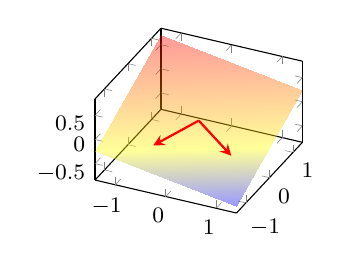
\begin{tikzpicture} 
\begin{axis}[footnotesize,font=\footnotesize,domain=-1.4:1.4
    ,axis equal image    ] 
    \addplot3[surf,shader=interp,samples=2,blue,opacity=0.4] {-x/6+y/3};
    \addplot3[red,thick,quiver={u=-0.51,v=-0.84,w=-0.20},-stealth] coordinates {(0,0,0)};
    \addplot3[red,thick,quiver={u=0.85,v=-0.44,w=-0.29},-stealth] coordinates {(0,0,0)};
\end{axis}
\end{tikzpicture} 
\quad
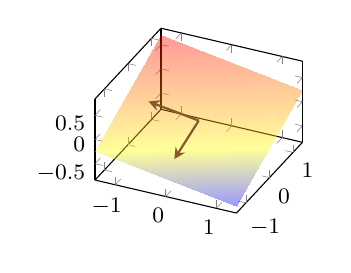
\begin{tikzpicture} 
\begin{axis}[footnotesize,font=\footnotesize,domain=-1.4:1.4
    ,axis equal image    ] 
    \addplot3[surf,shader=interp,samples=2,blue,opacity=0.4] {-x/6+y/3};
    \addplot3[brown!70!black,thick,quiver={u=-0.99,v=-0.01,w=0.16},-stealth] coordinates {(0,0,0)};
    \addplot3[brown!70!black,thick,quiver={u=-0.04,v=-0.95,w=-0.31},-stealth] coordinates {(0,0,0)};
\end{axis}
\end{tikzpicture} 
\end{center}
Similarly in other dimensions for other subspaces.
Just as~\(\RR^n\) is called \(n\)-dimensional and has \(n\)~standard unit vectors, so we analogously define the dimension of any subspace.

\begin{definition} \label{def:dim} 
Let \WW\ be a \idx{subspace} of~\(\RR^n\). 
The number of vectors in an \idx{orthonormal basis} for~\WW\ is called the \bfidx{dimension} of~\WW, denoted~\(\dim\WW\).
By convention, \(\dim\{\ov\}=0\)\,.
\end{definition}

\begin{example} \label{eg:}
\begin{itemize}
\item \autoref{eg:orthbas1} finds that the linear subspace \(x=y=z\) is spanned by the orthonormal basis \(\{(1/{\sqrt3},1/{\sqrt3},1/{\sqrt3})\}\).  
With one vector in the basis, the line is one dimensional.

\item \autoref{eg:orthbas2} finds that the planar subspace \(-x+2y-2z=0\) is spanned by the orthonormal basis \(\{\uv_1,\uv_2\}\) where \(\uv_1=(-\frac23,\frac13,\frac23)\), and \(\uv_2=(\frac23,\frac23,\frac13)\).  
With two vectors in the basis, the plane is two dimensional.

\item  Subspace \(\WW=\Span\{(5,1,-1/2),(0,-3,-1),(-4,1,1)\}\) of \autoref{eg:orthospan} is found to have an orthonormal basis of the vectors  \((-0.99,-0.01,0.16)\) and \((-0.04,-0.95,-0.31)\).
With two vectors in the basis, the subspace is two dimensional; that is, \(\dim\WW=2\)\,.

\item Since the subspace~\(\RR^n\) (\autoref{eg:somsubsg}) has an orthonormal basis of the \(n\)~standard unit vectors, \(\{\hlist\ev n\}\), then  \(\dim\RR^n=n\)\,.

\item The \idx{El Nino} windowed data of \autoref{eg:orthbapp} is effectively spanned by four orthonormal vectors.  Despite the apparent complexity of the signal, the data effectively lies in a subspace of dimension four (that of two oscillators).
\end{itemize}
\end{example}


\begin{theorem} \label{thm:rowcolD} 
The \idx{row space} and \idx{column space} of a matrix~\(A\) have the same \idx{dimension}.
Further, given an \svd\ of the matrix, say \(A=\usv\), an \idx{orthonormal basis} for the column space is the first \(\rank A\)~columns of~\(U\), and that for the row space is the first \(\rank A\)~columns of~\(V\).
\end{theorem}

\begin{proof} 
From \autoref{def:mattran} of the transpose, the rows of~\(A\) are the same as the columns of~\(\tr A\), and so the row space of~\(A\) is the same as the column space of~\(\tr A\).  
Hence,
\begin{align*}
&\text{dimension of the row space of }A
\\&=\text{dimension of the column space of }\tr A
\\&=\rank(\tr A) \quad(\text{by Proc.~\ref{pro:ospan}})
\\&=\rank A \quad(\text{by \autoref{thm:ranktr}})
\\&=\text{dimension of the column space of }A
\quad(\text{by Proc.~\ref{pro:ospan}}).
\end{align*}
%Hence the row space and the column space have the same dimension.

Let \(m\times n\) matrix~\(A\) have an \svd\ \(A=\usv\) and \(r=\rank A\).
Then \autoref{pro:ospan} establishes that an orthonormal basis for the column space of~\(A\) is the first \(r\)~columns of~\(U\).
Recall that \(\tr A=\tr{(\usv)} =V\tr S\tr U\) is an \svd\ for~\(\tr A\) (\autoref{thm:ranktr}) and so an orthonormal basis for the column space of~\(\tr A\) is the first \(r\)~columns of~\(V\) (\autoref{pro:ospan}).
Since the row space of~\(A\) is the column space of~\(\tr A\), an orthonormal basis for the row space of~\(A\) is the first \(r\)~columns of~\(V\).
\end{proof}


\begin{example} \label{eg:2x2rcsp}
Find an \svd\ of the matrix~\(A=\begin{bmatrix} 1&-4\\1/2&-2 \end{bmatrix}\) and compare the column space and the row space of the matrix.
\begin{solution} 
Ask \script\ for an \svd\ and interpret:
\begin{verbatim}
A=[1 -4; 1/2 -4]
[U,S,V]=svd(A)
\end{verbatim}
\setbox\ajrqrbox\hbox{\qrcode{% orthonormal basis
A=[1 -4; 1/2 -4]
[U,S,V]=svd(A)
}}%
\marginpar{\usebox{\ajrqrbox}}%
computes the \svd\ 
\begin{verbatim}
U =
  -0.8944  -0.4472
  -0.4472   0.8944
S =
   4.6098        0
        0   0.0000
V =
  -0.2425   0.9701
   0.9701   0.2425
\end{verbatim}
There is one non-zero singular value---the matrix has rank one---so an orthonormal basis for the column space is the first column of matrix~\(U\), namely \((-0.89,-0.45)\) \twodp.

\marginpar{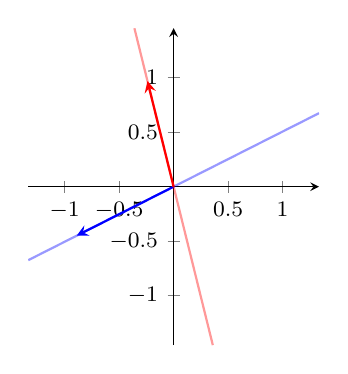
\begin{tikzpicture} 
\begin{axis}[small,font=\footnotesize,domain=-1.5:1.5
%    ,width=16em
    ,axis equal image, axis lines=middle    ] 
    \addplot[samples=2,blue,opacity=0.4,thick] ({-0.89*x},{-0.45*x});
    \addplot[blue,thick,quiver={u=-0.89,v=-0.45},-stealth] coordinates {(0,0)};
    \addplot[samples=2,red,opacity=0.4,thick] ({-0.24*x},{0.97*x});
    \addplot[red,thick,quiver={u=-0.24,v=0.97},-stealth] coordinates {(0,0)};
\end{axis}
\end{tikzpicture}}%
Complementing this, as there is one non-zero singular value---the matrix has rank one---so an orthonormal basis for the row space is the first column of matrix~\(V\), namely \((-0.24,0.97)\).
As illustrated in the margin, the two subspaces, the row space (red) and the column space (blue), are different but of the same dimension.
(As in general, here the row and column spaces are not orthogonal.)
\end{solution}
\end{example}



\begin{activity}
Using the \svd\ of \autoref{eg:2x2rcsp}, what is the dimension of the \idx{nullspace} of the matrix~\(\begin{bmatrix} 1&-4\\1/2&-2 \end{bmatrix}\)?
\actposs[4]1230
%\partswidth=5em
%\begin{parts}
%\item 0
%\item 1
%\item 2
%\item 3
%\end{parts}
\end{activity}


\begin{example} \label{eg:}
Use the \svd\ of the matrix~\(B\) in \autoref{eg:orthospan} to compare the column space and the row space of matrix~\(B\).
\begin{solution} 
Recall that there are two non-zero singular values---the matrix has rank two---so an orthonormal basis for the column space is  the first two columns of matrix~\(U\), namely the vectors  \((-0.99,-0.01,0.16)\) and \((-0.04,-0.95,-0.31)\).

Complementing this, as there are two non-zero singular values---the matrix has rank two---so an orthonormal basis for the row space is the set of the first two columns of matrix~\(V\), namely the vectors  \((-0.78,-0.02, 0.63)\) and \((-0.28, 0.91,-0.32)\).
As illustrated below in stereo, the two subspaces, the row space~(red) and the column space~(blue), are different but of the same dimension.
\begin{center}
\qview{58}{62}{\begin{tikzpicture} 
\begin{axis}[small,font=\footnotesize,domain=-1.4:1.4
    ,axis equal image,view={\q}{20}    ] 
    \addplot3[surf,samples=2,blue,opacity=0.3] {-x/6+y/3};
    \addplot3[blue,thick,quiver={u=-0.99,v=-0.01,w=0.16},-stealth] coordinates {(0,0,0)};
    \addplot3[blue,thick,quiver={u=-0.04,v=-0.95,w=-0.31},-stealth] coordinates {(0,0,0)};
    \addplot3[surf,samples=2,red,opacity=0.3] {-0.8*x-0.6*y};
    \addplot3[red,thick,quiver={u=-0.78,v=-0.02,w=0.63},-stealth] coordinates {(0,0,0)};
    \addplot3[red,thick,quiver={u=-0.28,v=0.91,w=-0.32},-stealth] coordinates {(0,0,0)};
\end{axis}
\end{tikzpicture}}
\end{center}
\end{solution}
\end{example}




\begin{definition} \label{def:nullity} 
The \bfidx{nullity} of a matrix~\(A\) is the \idx{dimension} of its \idx{nullspace} (defined in \autoref{thm:homosubsp}), and is denoted by \(\nullity(A)\).
\end{definition}

\begin{example} \label{eg:}
\autoref{eg:nullsp} finds the nullspace of the two matrices
\begin{equation*}
\begin{bmatrix} 3&-3\\-1&-7 \end{bmatrix}
\quad\text{and}\quad
\begin{bmatrix} 1&2&4&-3\\
1&2&-3&6 \end{bmatrix}.
\end{equation*}
\begin{itemize}
\item The first matrix has nullspace~\(\{\ov\}\) which has dimension zero and hence the nullity of the matrix is zero.
\item The second matrix, \(2\times4\), has nullspace written as \(\Span\{(-2,1,0,0)\clb(-\frac{15}7,0,\frac97,1)\}\).
Being spanned by two vectors not proportional to each other, we expect the dimension of the nullspace, the nullity, to be two.
To check, compute the singular values of the matrix whose columns are these vectors: calling the matrix~\(N\) for nullspace,
\begin{verbatim}
N=[-2 1 0 0; -15/7 0 9/7 1]'
svd(N)
\end{verbatim}
\setbox\ajrqrbox\hbox{\qrcode{% dimension
N=[-2 1 0 0; -15/7 0 9/7 1]'
svd(N)
}}%
\marginpar{\usebox{\ajrqrbox}}%
which computes the singular values
\begin{verbatim}
   3.2485
   1.3008
\end{verbatim}
Since there are two non-zero singular values, there are two orthonormal vectors spanning the subspace, the nullspace, hence its dimension, the nullity, is two.
\end{itemize}
\end{example}



\begin{example} \label{eg:nullitysvd}
For the matrix
\begin{equation*}
C=\begin{bmatrix} -1&-2&2&1
\\-3&3&1&0
\\2&-5&1&1 \end{bmatrix},
\end{equation*}
find an orthonormal basis for its nullspace and hence determine its nullity.
\begin{solution} 
To find the nullspace construct a general solution to the homogeneous system \(C\xv=\ov\) with \autoref{pro:gensol}.
\begin{enumerate}
\item Enter  into \script\ the matrix~\(C\) and compute an \svd\ via \verb|[U,S,V]=svd(C)| to find \twodp
\setbox\ajrqrbox\hbox{\qrcode{% nullity
C=[-1 -2 2 1
 -3 3 1 0
 2 -5 1 1]
[U,S,V]=svd(C)
}}%
\marginpar{\usebox{\ajrqrbox}}%
\begin{verbatim}
U =
   0.24   0.78  -0.58
  -0.55   0.60   0.58
   0.80   0.18   0.58
S =
   6.95      0      0      0
      0   3.43      0      0
      0      0   0.00      0
V =
   0.43  -0.65   0.63  -0.02
  -0.88  -0.19   0.42   0.10
   0.11   0.68   0.62  -0.37
   0.15   0.28   0.21   0.92
\end{verbatim}
\item Since the right-hand side of \(C\xv=\ov\) is zero the solution to \(U\zv=\ov\) is \(\zv=\ov\)\,.
\item Then, because the rank of the matrix is two, the solution to \(S\yv=\zv=\ov\) is \(\yv=(0,0,y_3,y_4)\) for free variables \(y_3\) and~\(y_4\).
\item The solution to \(\tr V\xv=\yv\) is \(\xv=V\yv=\vv_3y_3+\vv_4y_4
=y_3(0.63,0.42,0.62,0.21)+y_4(-0.02,0.10,-0.37,0.92)\).
\end{enumerate}
Hence  \(\Span\{(0.63,0.42,0.62,0.21),\,(-0.02,0.10,-0.37,0.92)\}\) is the nullspace of matrix~\(C\).
Because the columns of~\(V\) are orthonormal, the two vectors appearing in this span are orthonormal and so form an orthonormal basis for the nullspace.
Hence \(\nullity C=2\)\,.
\end{solution}
\end{example}



This \autoref{eg:nullitysvd} indicates that the nullity is determined by the number of zero columns in the diagonal matrix~\(S\) of an \svd.
Conversely, the rank of a matrix is determined by the number of non-zero columns in the diagonal matrix~\(S\) of an \svd.
Put these two facts together in general and we get the following theorem that helps characterise solutions of linear equations.





\begin{theorem}[\bfidx{rank theorem}] \label{thm:rank} 
For every \(m\times n\) matrix~\(A\),  \(\rank A+\nullity A=n\)\,, the number of columns of~\(A\).
\end{theorem}
\begin{proof} 
Set \(r=\rank A\)\,.
By \autoref{pro:gensol} a general solution to the homogeneous system \(A\xv=\ov\) involves \(n-r\) free variables \(y_{r+1},\ldots,y_n\) in the linear combination form \(\vv_{r+1}y_{r+1}+\cdots +\vv_ny_n\)\,.  
Hence the nullspace is \(\Span\{\vv_{r+1},\ldots,\vv_n\}\).
Because matrix~\(V\) is orthogonal, the vectors \(\vv_{r+1},\ldots,\vv_n\) are orthonormal; that is, they form an orthonormal basis for the nullspace, and so the nullspace is of dimension~\(n-r\)\,.
Consequently, \(\rank A+\nullity A=r+(n-r)=n\)\,.
\end{proof}


\begin{example} \label{eg:}
Compute \svd{}s to determine the rank and nullity of each of the given matrices.
%for i=1:999,a=round(randn(ceil(1+4*rand(1,2)))*2);if rank(a)<min(size(a)), A=a, svd(A), break, end,end
\begin{enumerate}
\item \(\begin{bmatrix} 1&-1&2
\\2&-2&4
 \end{bmatrix}\)
\begin{solution} 
Enter the matrix into \script\ and compute the singular values:
\begin{verbatim}
A=[1 -1 2
2 -2 4]
svd(A)
\end{verbatim}
\setbox\ajrqrbox\hbox{\qrcode{% rank
A=[1 -1 2
2 -2 4]
svd(A)
}}%
\marginpar{\usebox{\ajrqrbox}}%
The resultant singular values are
\begin{verbatim}
   5.4772
   0.0000
\end{verbatim}
The one non-zero singular value indicates \(\rank A=1\)\,.
Since the matrix has three columns, the nullity---the dimension of the nullspace---is \(3-1=2\)\,. 
\end{solution}
 
\item \(\begin{bmatrix} 1&-1&-1
\\1&0&-1
\\-1&3&1 \end{bmatrix}\)
\begin{solution} 
Enter the matrix into \script\ and compute the singular values:
\begin{verbatim}
B=[1 -1 -1
1 0 -1
-1 3 1]
svd(B)
\end{verbatim}
\setbox\ajrqrbox\hbox{\qrcode{% rank
B=[1 -1 -1
1 0 -1
-1 3 1]
svd(B)
}}%
\marginpar{\usebox{\ajrqrbox}}%
The resultant singular values are
\begin{verbatim}
   3.7417
   1.4142
   0.0000
\end{verbatim}
The two non-zero singular values indicate  \(\rank B=2\)\,.
Since the matrix has three columns, the nullity---the dimension of the nullspace---is \(3-2=1\)\,. 
\end{solution}


\item \(\begin{bmatrix} 0&0&-1&-3&2
\\-2&-2&1&0&1
\\1&-1&2&8&-2
\\-1&1&0&-2&-2
\\-3&-1&0&-5&1 \end{bmatrix}\)
\begin{solution} 
Enter the matrix into \script\ and compute the singular values:
\begin{verbatim}
C=[0 0 -1 -3 2
 -2 -2 1 -0 1
  1 -1 2 8 -2
 -1 1 -0 -2 -2
 -3 -1 -0 -5 1]
svd(C)
\end{verbatim}
\setbox\ajrqrbox\hbox{\qrcode{% rank
C=[0 0 -1 -3 2
 -2 -2 1 -0 1
 1 -1 2 8 -2
 -1 1 -0 -2 -2
 -3 -1 -0 -5 1]
svd(C)
}}%
\marginpar{\usebox{\ajrqrbox}}%
The resultant singular values are
\begin{verbatim}
   10.8422
    4.0625
    3.1532
    0.0000
    0.0000
\end{verbatim}
Three non-zero singular values indicate \(\rank C=3\)\,.
Since the matrix has five columns, the nullity---the dimension of the nullspace---is \(5-3=2\)\,. 
\end{solution}


%\item \(\begin{bmatrix} 0&0&-1&-3&2
%\\-2&-2&1&0&1
%\\1&-4&1&-2&1
%\\-1&1&0&-2&-2
%\\-3&-1&0&-5&1 \end{bmatrix}\)
\end{enumerate}
\end{example}



\begin{activity}
The matrix
\begin{equation*}
\begin{bmatrix} -2&1&4&0&-4
\\-1&1&0&-2&0
\\-3&1&3&2&-3
\\0&0&1&0&-1 \end{bmatrix}
\text{ has singular values}\quad
\begin{matrix}\tt 8.1975
\\\tt 2.6561
\\\tt 1.6572
\\\tt 0.0000 \end{matrix}
\end{equation*}
computed with \verb|svd()|.
What is its nullity?
\actposs[4]2310
%\partswidth=5em
%\begin{parts}
%\item 0
%\item 1
%\item 2
%\item 3
%\end{parts}
\end{activity}





\begin{example} \label{eg:}
Each of the following graphs plot all the column vectors of a matrix. What is the nullity of each of the matrices?  Give reasons.
\begin{enumerate}
\item 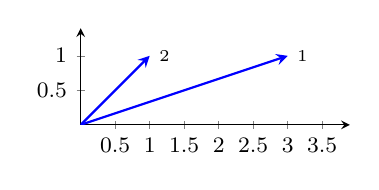
\begin{tikzpicture} 
\begin{axis}[footnotesize,font=\footnotesize
    ,xmax=3.9,ymax=1.4
    ,axis equal image, axis x line=middle, axis y line= middle ] 
    \addplot[blue,thick,quiver={u=3,v=1},-stealth] coordinates {(0,0)};
    \node[right] at (axis cs:3,1) {$\av_1$};
    \addplot[blue,thick,quiver={u=1,v=1},-stealth] coordinates {(0,0)};
    \node[right] at (axis cs:1,1) {$\av_2$};
\end{axis}
\end{tikzpicture}
\begin{solution} 
Zero.
These two column vectors in the plane must come from a \(2\times2\) matrix~\(A\).
Since the two columns are at a non-trivial angle, every point in the plane may be written as a linear combination of \(\av_1\) and~\(\av_2\), hence the column space of~\(A\) is~\(\RR^2\).
Consequently, \(\rank A=2\)\,. 
From the rank theorem: \(\nullity A=n-\rank A=2-2=0\)\,. 
\end{solution}


\item 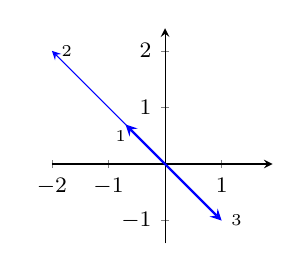
\begin{tikzpicture} 
\begin{axis}[footnotesize,font=\footnotesize
    ,xmax=1.9,ymax=2.4,ymin=-1.4
    ,axis equal image, axis x line=middle, axis y line= middle ] 
    \addplot[blue,thick,quiver={u=-0.7,v=0.7},-stealth] coordinates {(0,0)};
    \node[left] at (axis cs:-0.5,0.5) {$\bv_1$};
    \addplot[blue,quiver={u=-2,v=2},-stealth] coordinates {(0,0)};
    \node[right] at (axis cs:-2,2) {$\bv_2$};
    \addplot[blue,thick,quiver={u=1,v=-1},-stealth] coordinates {(0,0)};
    \node[right] at (axis cs:1,-1) {$\bv_3$};
\end{axis}
\end{tikzpicture}
\begin{solution} 
Two.
These three column vectors in the plane must come from a \(2\times3\) matrix~\(B\).
The three vectors are all in a line, so the column space of matrix~\(B\) is a line.
Consequently, \(\rank B=1\)\,. 
From the rank theorem: \(\nullity B=n-\rank B=3-1=2\)\,. 
\end{solution}


\item 
\qview{30}{35} {
\begin{tikzpicture} 
\begin{axis}[small,font=\footnotesize,view={\q}{30}
    ,xmax=2.9,ymax=2.9,zmax=2.9,xmin=-2.9
    ,axis equal image ]
    \addplot3[blue,thick,quiver={u=1,v=2,w=-2},-stealth] coordinates {(0,0,0)};
    \node[right] at (axis cs:1,2,-2) {$\cv_1$};
    \addplot3[blue,thick,quiver={u=-2,v=2,w=1},-stealth] coordinates {(0,0,0)};
    \node[above] at (axis cs:-2,2,1) {$\cv_2$};
    \addplot3[blue,thick,quiver={u=2,v=1,w=2},-stealth] coordinates {(0,0,0)};
    \node[above] at (axis cs:2,1,2) {$\cv_3$};
    \addplot3[blue,thick,quiver={u=0,v=-2,w=0},-stealth] coordinates {(0,0,0)};
    \node[below] at (axis cs:0,-2,0) {$\cv_4$};
\end{axis}
\end{tikzpicture}}
a \idx{stereo pair}.
\begin{solution} 
One.
These four column vectors in 3D space must come from a \(3\times4\) matrix~\(C\).
Since the four columns do not all lie in a line or plane, every point in space may be written as a linear combination of \(\hlist\cv 4\), hence the column space of~\(C\) is~\(\RR^3\).
Consequently, \(\rank C=3\)\,. 
From the rank theorem: \(\nullity C=n-\rank C=4-3=1\)\,. 
\end{solution}

\item 
\qview{30}{35} {
\begin{tikzpicture} 
\begin{axis}[small,font=\footnotesize,view={\q}{30}
    ,axis equal image  ]
    \addplot3[surf,shader=interp,samples=2,opacity=0.4] {-x/5+2*y/5};
    \addplot3[blue,thick,quiver={u=4,v=2,w=0},-stealth] coordinates {(0,0,0)};
    \node[right] at (axis cs:4,2,0) {$\dv_1$};
    \addplot3[blue,thick,quiver={u=0,v=5,w=2},-stealth] coordinates {(0,0,0)};
    \node[right] at (axis cs:0,5,2) {$\dv_2$};
    \addplot3[blue,thick,quiver={u=-5,v=0,w=1},-stealth] coordinates {(0,0,0)};
    \node[below] at (axis cs:-5,0,1) {$\dv_3$};
    \addplot3[blue,thick,quiver={u=3,v=-1,w=-1},-stealth] coordinates {(0,0,0)};
    \node[below] at (axis cs:3,-1,-1) {$\dv_4$};
\end{axis}
\end{tikzpicture}}
a \idx{stereo pair}.
\begin{solution} 
Two.
These four column vectors in 3D space must come from a \(3\times4\) matrix~\(D\).
Since the four columns all lie in a plane (as suggested by the drawn plane), and linear combinations can give every point in the plane, hence the column space of~\(D\) has dimension two.
Consequently, \(\rank D=2\)\,. 
The rank theorem gives \(\nullity D=n-\rank D=4-2=2\)\,. 
\end{solution}

\end{enumerate}
\end{example}


The recognition of these new concepts associated with matrices and linear equations, then empowers us to extend the list of exact properties that ensure a system of linear equations has a unique solution. 

\begin{theorem}[Unique Solutions: version~2]  \label{thm:ftim2} 
For every \(n\times n\) \idx{square matrix}~\(A\), and extending \autoref{thm:ftim1}, the following statements are equivalent:
\begin{enumerate}
\item\label{thm:ftim2i} \(A\) is \idx{invertible};
\item\label{thm:ftim2ii} \(A\xv=\bv\) has a \idx{unique solution} for every \(\bv\in\RR^n\);
\item\label{thm:ftim2iii} \index{homogeneous}\(A\xv=\ov\) has only the zero solution;
\item\label{thm:ftim2iv} all \(n\)~\idx{singular value}s of~\(A\) are nonzero;
\item\label{thm:ftim2ivx} the \idx{condition number} of~\(A\) is finite (\(\verb|rcond|>0\));
\item\label{thm:ftim2v} \(\rank A=n\)\,;
\item\label{thm:ftim2vi} \(\nullity A=0\)\,;
\item\label{thm:ftim2vii} the \idx{column vector}s of~\(A\) span~\(\RR^n\);
\item\label{thm:ftim2viii} the \idx{row vector}s of~\(A\) span~\(\RR^n\).
\end{enumerate}
\end{theorem}
\begin{proof} 
\autoref{thm:ftim1} establishes the equivalence of the statements~\ref{thm:ftim2i}--\ref{thm:ftim2v}.  
We prove the equivalence of these with the statements~\ref{thm:ftim2vi}--\ref{thm:ftim2viii}.
\begin{description}
\item[\ref{thm:ftim2v}$\iff$\ref{thm:ftim2vi}]
The Rank \autoref{thm:rank} assures us that \(\nullity A=0\) if and only if \(\rank A=n\)\,.
\item[\ref{thm:ftim2ii}$\implies$\ref{thm:ftim2vii}] 
By~\ref{thm:ftim2ii} every \(\bv\in\RR^n\) can be written as \(\bv=A\xv\)\,. But \(A\xv\)~is a linear combination of the columns of~\(A\) and so \(\bv\)~is in the span of the columns.  
Hence the column vectors of~\(A\) span~\(\RR^n\).
\item[\ref{thm:ftim2vii}$\implies$\ref{thm:ftim2v}] 
Suppose \(\rank A=r\) reflecting \(r\)~non-zero singular values in an \svd\ \(A=\usv\).
\autoref{pro:ospan} assures us the column space of~\(A\) has  orthonormal basis~\(\{\hlist\uv r\}\).
But the column space is~\(\RR^n\) (statement~\ref{thm:ftim2vii}) which also has the orthonormal basis of the \(n\)~standard unit vectors.
\autoref{thm:sameD} assures us that the number of basis vectors must be the same; that is, \(\rank A=r=n\)\,.
\item[\ref{thm:ftim2v}$\iff$\ref{thm:ftim2viii}] 
\autoref{thm:ranktr} asserts \(\rank(\tr A)=\rank A\),  so the statement~\ref{thm:ftim2v} implies \(\rank(\tr A)=n\), and so statement~\ref{thm:ftim2vii} asserts the columns of~\(\tr A\) span~\(\RR^n\).
But the columns of~\(\tr A\)\ are the rows of~\(A\) so the rows of~\(A\) span~\(\RR^n\).
Conversely, if the rows of~\(A\) span~\(\RR^n\), then so do the columns of~\(\tr A\), hence \(\rank(\tr A)=n\) which by \autoref{thm:ranktr} implies \(\rank A=n\)\,.
\end{description}
\end{proof}



\index{dimension|)}





\sectionExercises



\begin{exercise} \label{ex:} 
Use your intuitive notion of a \idx{subspace} to decide whether each of the following drawn sets (3D in stereo pair) is a subspace, or not.

\begin{parts}
\item 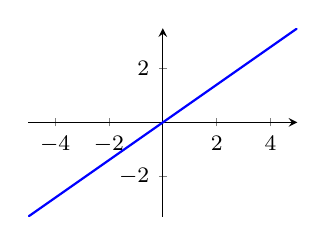
\begin{tikzpicture} 
\begin{axis}[footnotesize,font=\footnotesize
    ,axis equal image, axis lines=middle] 
    \addplot[blue,thick] {x*0.7};
\end{axis}
\end{tikzpicture}
\answer{Subspace.}

\item 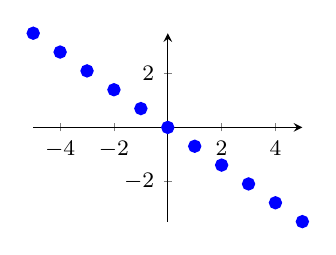
\begin{tikzpicture} 
\begin{axis}[footnotesize,font=\footnotesize
    ,axis equal image, axis lines=middle] 
    \addplot[blue,thick,mark=*,samples=11,only marks] {-x*0.7};
\end{axis}
\end{tikzpicture}
\answer{Not a subspace.}

\item 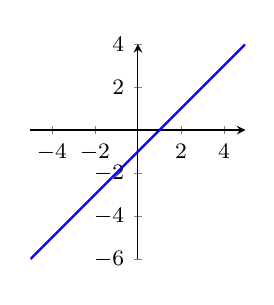
\begin{tikzpicture} 
\begin{axis}[footnotesize,font=\footnotesize
    ,axis equal image, axis lines=middle ] 
    \addplot[blue,thick] {-1+x};
\end{axis}
\end{tikzpicture}
\answer{Not a subspace.}


\item 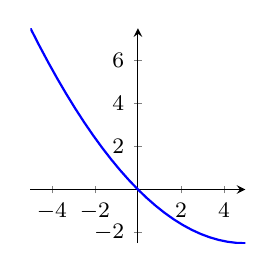
\begin{tikzpicture} 
\begin{axis}[footnotesize,font=\footnotesize
    ,axis equal image, axis lines=middle ] 
    \addplot[blue,thick] {-x+x^2/10};
\end{axis}
\end{tikzpicture}
\answer{Not a subspace.}

\item 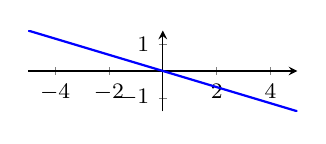
\begin{tikzpicture} 
\begin{axis}[footnotesize,font=\footnotesize
    ,axis equal image, axis lines=middle] 
    \addplot[blue,thick] {-x*0.3};
\end{axis}
\end{tikzpicture}
\answer{Subspace.}


\item 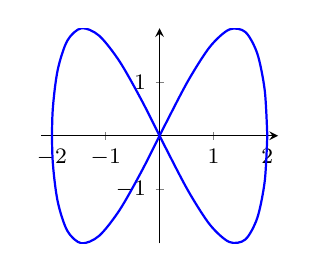
\begin{tikzpicture} 
\begin{axis}[footnotesize,font=\footnotesize,xmin=-2.2,xmax=2.2
    ,axis equal image, axis lines=middle ] 
    \addplot[blue,smooth,samples=30,domain=0:360,thick] ({2*cos(x)},{2*sin(2*x)});
\end{axis}
\end{tikzpicture}
\answer{Not a subspace.}

\item 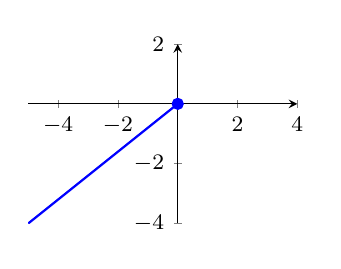
\begin{tikzpicture} 
\begin{axis}[footnotesize,font=\footnotesize,xmax=4,ymax=2
    ,axis equal image, axis lines=middle ] 
    \addplot[blue,thick,domain=-5:0] {x*0.8};
    \addplot[only marks,blue] coordinates {(0,0)};
\end{axis}
\end{tikzpicture}
\answer{Not a subspace.}

\item \begin{tikzpicture} 
\begin{axis}[footnotesize,font=\footnotesize
    ,axis equal, axis lines=middle,ymax=4,ymin=-4] 
    \addplot[blue,thick] {4*x};
\end{axis}
\end{tikzpicture}
\answer{Subspace.}

\setcounter{i}{\value{enumii}}
\end{parts}\begin{enumerate}
\setcounter{enumii}{\value{i}}

\item \qview{28}{32}{\begin{tikzpicture} 
\begin{axis}[footnotesize,font=\footnotesize
    ,axis equal image ,view={\q}{25}   ] 
    \addplot3[blue,samples y=0,thick] ({x*0.8},{x},{-0.6*x});
    \addplot3[only marks,black] coordinates {(0,0,0)};
\end{axis}
\end{tikzpicture}}
\answer{Subspace.}

\item \qview{28}{32}{\begin{tikzpicture} 
\begin{axis}[footnotesize,font=\footnotesize
    ,axis equal image ,view={\q}{30}   ] 
    \addplot3[blue,samples y=0,thick] ({x-x^3/100},{x},{0.1*x^2});
    \addplot3[only marks,black] coordinates {(0,0,0)};
\end{axis}
\end{tikzpicture}}
\answer{Not a subspace.}

\item \qview{28}{32}{\begin{tikzpicture} 
\begin{axis}[footnotesize,font=\footnotesize
    ,axis equal image ,view={\q}{25}   ] 
    \addplot3[blue,samples y=0,thick,only marks,samples=11] ({-x*0.8},{x},{0.6*x});
    \addplot3[only marks,black] coordinates {(0,0,0)};
\end{axis}
\end{tikzpicture}}
\answer{Not a subspace.}

\item \qview{28}{32}{\begin{tikzpicture} 
\begin{axis}[footnotesize,font=\footnotesize
    ,axis equal image  ,view={\q}{30}  ] 
    \addplot3[only marks,black] coordinates {(0,0,0)};
    \addplot3[surf,shader=interp,samples=2,opacity=0.6] {x/3+y/6};
\end{axis}
\end{tikzpicture}}
\answer{Subspace.}

\item \qview{28}{32}{\begin{tikzpicture} 
\begin{axis}[footnotesize,font=\footnotesize
    ,axis equal image  ,view={\q}{30}  ] 
    \addplot3[only marks,black] coordinates {(0,0,0)};
    \addplot3[surf,shader=interp,samples=2,opacity=0.6] {4+x/3+y/6};
\end{axis}
\end{tikzpicture}}
\answer{Not a subspace.}

\item \qview{28}{32}{\begin{tikzpicture} 
\begin{axis}[footnotesize,font=\footnotesize
    ,axis equal image, width=13em    ] 
    \addplot3[only marks,black] coordinates {(0,0,0)};
    \addplot3[surf,opacity=0.5] {-x^3/100+y/4};
\end{axis}
\end{tikzpicture}}
\answer{Not a subspace.}

\item \qview{28}{32}{\begin{tikzpicture} 
\begin{axis}[footnotesize,font=\footnotesize
    ,axis equal image  ,view={\q}{30}  ] 
    \addplot3[only marks,black] coordinates {(0,0,0)};
    \addplot3[surf,shader=interp,samples=2,opacity=0.6] {-x/3+y/6};
\end{axis}
\end{tikzpicture}}
\answer{Subspace.}

\item \qview{28}{32}{\begin{tikzpicture} 
\begin{axis}[footnotesize,font=\footnotesize
    ,axis equal image, width=13em    ] 
    \addplot3[only marks,black] coordinates {(0,0,0)};
    \addplot3[surf,opacity=0.5] {-x/4+y^2/20};
\end{axis}
\end{tikzpicture}}
\answer{Not a subspace.}

\end{enumerate}
\end{exercise}





\begin{exercise} \label{ex:} 
Use \autoref{def:subspace} to decide whether each of the following is a \idx{subspace}, or not.  Give reasons.
\begin{enumerate}
\item All vectors in the line \(y=2x\)\,.
\answer{Subspace.}

\item All vectors in the line \(3.2y=0.8x\)\,.
\answer{Subspace.}

\item All vectors \((x,y)=(t,2+t)\) for all real~\(t\).
\answer{Not a subspace.}

\item All vectors \((1.3n,-3.4n)\) for all integer~\(n\).
\answer{Not a subspace.}

\item All vectors \((x,y)=(-3.3-0.3t,2.4-1.8t)\) for all real~\(t\).%
\answer{Not a subspace.}

\item \(\Span\{(6,-1),(1,2)\}\)
\answer{Subspace.}

\item All vectors \((x,y)=(6-3t,t-2)\) for all real~\(t\).
\answer{Subspace.}

\item The vectors \((2,1,-3)t+(5,-\frac12,2)s\) for all real \(s,t\).
\answer{Subspace.}

\item The vectors \((0.9,2.4,1)t-(0.2,0.6,0.3)s\) for all real \(s,t\).
\answer{Subspace.}

\item All vectors \((x,y)\) such that \(y=x^3\).
\answer{Not a subspace.}

\item All vectors \((x,y,z)\) such that \(x=2t\)\,, \(y=t^2\) and \(z=t/2\) for all~\(t\).
\answer{Not a subspace.}

\item The vectors \((t,n,2t+3n)\) for real~\(t\) and integer~\(n\).
\answer{Not a subspace.}

\item \(\Span\{(0,-1,1),(-1,0,2)\}\)
\answer{Subspace.}

\item The vectors \((2.7,2.6,-0.8,2.1)s+(0.5,0.1,-1,3.3)t\) for all real~\(s,t\).
\answer{Subspace.}

\item The vectors \((1.4,2.3,1.5,4)+(1.2,-0.8,-1.2,2)t\) for all real~\(t\).
\answer{Not a subspace.}

\item The vectors \((t^3,2t^3)\) for all real~\(t\) (tricky).
\answer{Subspace.}

\item The vectors \((t^2,3t^2)\) for all real~\(t\) (tricky).
\answer{Not a subspace.}

\end{enumerate}
\end{exercise}





\begin{exercise} \label{ex:} 
Let \(\WW_1\)\ and~\(\WW_2\) be any two \idx{subspace}s of~\(\RR^n\) (\autoref{def:subspace}).  
\begin{enumerate}
\item Use the definition to prove that the intersection of \(\WW_1\)\ and~\(\WW_2\) is also a subspace of~\(\RR^n\).
\item Give an example to prove that the union of \(\WW_1\)\ and~\(\WW_2\) is not necessarily a subspace of~\(\RR^n\).
\end{enumerate}
\end{exercise}





\begin{exercise} \label{ex:} 
For each of the following matrices, partially solve linear equations to determine whether the given vector~\(\bv_j\) is in the \idx{column space}, and to determine if the given vector~\(\rv_j\) is in the \idx{row space} of the matrix.
Work small problems by hand, and address larger problems with \script.
Record your working or \script\ commands and output.
% A=round(randn(m,n)*3)+0, b=round(randn(m,1)*3)+0, c=round(randn(n,1)*3)+0, rref([A b]), rref([A' c])
\begin{enumerate}
\item \(\eAii=\begin{bmatrix} 2&1
\\5&4 \end{bmatrix}\),
\(\bv_{\arabic{enumii}}=\begin{bmatrix} 3
\\-2 \end{bmatrix}\),
\(\rv_{\arabic{enumii}}=\begin{bmatrix} 1
\\0 \end{bmatrix}\)
\answer{\(\bv_{\arabic{enumii}}\) is in column space;
\(\rv_{\arabic{enumii}}\)~is in row space.}

\item \(\eAii=\begin{bmatrix} -2&1
\\4&-2 \end{bmatrix}\),
\(\bv_{\arabic{enumii}}=\begin{bmatrix} 1
\\-3 \end{bmatrix}\),
\(\rv_{\arabic{enumii}}=\begin{bmatrix} 0\\0 \end{bmatrix}\)
\answer{\(\bv_{\arabic{enumii}}\) is not in column space;
\(\rv_{\arabic{enumii}}\)~is in row space.}

\item \(\eAii=\begin{bmatrix} 1&-1
\\-3&4
\\-3&5 \end{bmatrix}\),
\(\bv_{\arabic{enumii}}=\begin{bmatrix} 5
\\0
\\-1 \end{bmatrix}\),
\(\rv_{\arabic{enumii}}=\begin{bmatrix} 0
\\1 \end{bmatrix}\)
\answer{\(\bv_{\arabic{enumii}}\) is not in column space;
\(\rv_{\arabic{enumii}}\)~is in row space.}

\item \(\eAii=\begin{bmatrix} -2&-4&-5
\\-6&-2&1 \end{bmatrix}\),
\(\bv_{\arabic{enumii}}=\begin{bmatrix} 3
\\1 \end{bmatrix}\),
\(\rv_{\arabic{enumii}}=\begin{bmatrix} 2
\\-6
\\-11 \end{bmatrix}\)
\answer{\(\bv_{\arabic{enumii}}\) is in column space;
\(\rv_{\arabic{enumii}}\)~is in row space.}

\item \(\eAii=\begin{bmatrix} 3&2&4
\\1&6&0
\\1&-2&2 \end{bmatrix}\),
\(\bv_{\arabic{enumii}}=\begin{bmatrix} 10
\\2
\\4 \end{bmatrix}\),
\(\rv_{\arabic{enumii}}=\begin{bmatrix} 0
\\-1
\\2 \end{bmatrix}\)
\answer{\(\bv_{\arabic{enumii}}\) is in column space;
\(\rv_{\arabic{enumii}}\)~is not in row space.}

\item \(\eAii=\begin{bmatrix} 0&-1&-4
\\-2&0&4
\\7&-1&-3
\\1&1&3 \end{bmatrix}\),
\(\bv_{\arabic{enumii}}=\begin{bmatrix} 2
\\3
\\1
\\3 \end{bmatrix}\),
\(\rv_{\arabic{enumii}}=\begin{bmatrix} 1
\\0
\\0 \end{bmatrix}\)
\answer{\(\bv_{\arabic{enumii}}\) is not in column space;
\(\rv_{\arabic{enumii}}\)~is in row space.}

\item \(\eAii=\begin{bmatrix} -2&-1&5&4
\\0&-3&1&-1
\\3&3&4&3 \end{bmatrix}\),
\(\bv_{\arabic{enumii}}=\begin{bmatrix} 1
\\2
\\-4 \end{bmatrix}\),
\(\rv_{\arabic{enumii}}=\begin{bmatrix} 0
\\-3
\\1
\\-1 \end{bmatrix}\)
\answer{\(\bv_{\arabic{enumii}}\) is in column space;
\(\rv_{\arabic{enumii}}\)~is in row space.}

\item \(\eAii=\begin{bmatrix} -2&1&1&-1
\\2&-2&-1&0
\\-2&1&1&-2
\\2&5&-1&-1 \end{bmatrix}\),
\(\bv_{\arabic{enumii}}=\begin{bmatrix} 2
\\-1
\\3
\\0 \end{bmatrix}\),
\(\rv_{\arabic{enumii}}=\begin{bmatrix} -1
\\-2
\\0
\\-1 \end{bmatrix}\)
\answer{\(\bv_{\arabic{enumii}}\) is in column space;
\(\rv_{\arabic{enumii}}\)~is not in row space.}

\item \(\eAii=\begin{bmatrix} 1.0&0.8&2.1&1.4
\\0.6&-0.1&2.1&1.8
\\0.1&-0.1&2.1&1.2
\\1.7&-1.1&-1.9&2.9 \end{bmatrix}\),
\(\bv_{\arabic{enumii}}=\begin{bmatrix} 4.3
\\1.2
\\0.5
\\0.3 \end{bmatrix}\),
\(\rv_{\arabic{enumii}}=\begin{bmatrix} 0.0
\\1.5
\\-0.5
\\1.0 \end{bmatrix}\)
\answer{\(\bv_{\arabic{enumii}}\) is in column space;
\(\rv_{\arabic{enumii}}\)~is in row space.}

\end{enumerate}
\end{exercise}


\begin{exercise} \label{ex:} 
In each of the following, is the given vector in the nullspace of the given matrix?
% A=round(randn(m,n)*3)+0, v=null(A);v=v/max(abs(v));[~,d]=rat(v);v=v*max(d(:)), w=round(randn(n,1)*3)+0,A*w
\begin{enumerate}
\item \(\eAii=\begin{bmatrix} -11&-2&5
\\-1&1&1 \end{bmatrix}\),
\(\evii=\begin{bmatrix} -7\\6\\-13 \end{bmatrix}\)
\answer{yes}

\item \(\eAii=\begin{bmatrix} 3&-3&2
\\1&1&-3 \end{bmatrix}\),
\(\evii=\begin{bmatrix} 1
\\1
\\1 \end{bmatrix}\)
\answer{no}

\item \(\eAii=\begin{bmatrix} -5&0&-2
\\-6&2&-2
\\0&-5&-1 \end{bmatrix}\),
\(\evii=\begin{bmatrix} -2
\\-1
\\5 \end{bmatrix}\)
\answer{yes}

\item \(\eAii=\begin{bmatrix} -3&-2&0&2
\\5&0&1&-2
\\4&-4&4&2 \end{bmatrix}\),
\(\evii=\begin{bmatrix} 6
\\1
\\-10
\\10 \end{bmatrix}\)
\answer{yes}

\item \(\eAii=\begin{bmatrix} -3&2&3&1
\\-3&-2&-1&4
\\6&1&-1&-1 \end{bmatrix}\),
\(\evii=\begin{bmatrix} 2
\\-4
\\1
\\-2 \end{bmatrix}\)
\answer{no}

\item \(\eAii=\begin{bmatrix} -4&-2&2&-2
\\2&-1&-2&1
\\0&2&1&0
\\0&0&-8&-2 \end{bmatrix}\),
\(\evii=\begin{bmatrix} 11
\\-2
\\4
\\-16 \end{bmatrix}\)
\answer{yes}

\end{enumerate}
\end{exercise}




\begin{exercise} \label{ex:} 
Given the \svd{}s of Exercises~\ref{ex:hsledvs} and~\ref{ex:csledvs}, write down an \idx{orthonormal basis} for the span of the following sets of vectors.
\begin{enumerate}
\item \((-\frac{9}{5},-4)\),\quad \((\frac{12}{5},-3)\)
\answer{\iv, \jv}

\item \((-0.96,-0.72)\),\quad \((1.28,0.96)\)
\answer{\((\frac{4}{5},\frac{3}{5})\)}

\item \((7,-22,-4)/39\),\quad \((-34,-38,-53)/78\)
\answer{\((-1,-2,-2)/3\), \((2,-2,1)/3\)}

\item \((4,4,2)/33\),\quad \((4,4,2)/11\),\quad \((6,6,3)/11\)
\answer{\((2,2,1)/3\)}

\item \((-\frac{2}{5},\frac{11}{9},\frac{31}{90},\frac{4}{9})\),\quad
\((-\frac{2}{5},\frac{11}{9},\frac{31}{90},\frac{4}{9})\),\quad
\((-\frac{26}{45},-\frac{1}{3},\frac{17}{90},-\frac{2}{9})\), \\
\((\frac{26}{45},\frac{1}{3},-\frac{17}{90},\frac{2}{9})\)
\answer{\((2,-8,-2,-3)/9\), \((8,2,-1,2)/9\)}

\end{enumerate}
\end{exercise}





\begin{exercise} \label{ex:ospanrcn} 
Given any \(m\times n\) matrix~\(A\).
\begin{enumerate}
\item Explain how \autoref{pro:ospan} uses an \svd\ to find an \idx{orthonormal basis} for the \idx{column space} of~\(A\).
\item How does the same \svd\ give the orthonormal basis \(\{\hlist\vv r\}\) for the \idx{row space} of~\(A\)?  Justify your answer.
\item Why does the same \svd\ also give the orthonormal basis \(\{\vv_{r+1},\ldots,\vv_n\}\) for the \idx{nullspace} of~\(A\)?  Justify.
\end{enumerate}
\end{exercise}




\begin{exercise} \label{ex:obcrn} 
For each of the following matrices, compute an \svd\ with \script, and then use the properties of \autoref{ex:ospanrcn} to write down an \idx{orthonormal basis} for the \idx{column space}, the \idx{row space}, and the \idx{nullspace} of the matrix.
(The bases, especially for the nullspace, may differ in detail depending upon your version of \script.)
% These are used in the next exercise also.
% u=round(randn(m,m)*2); v=round(randn(n,n)*2); r=ceil(rand*min(m,n)), A=u*diag(round(randn(r,1)*2),m,n)*v', [U,S,V]=svd(A), col=U(:,1:r)', row=V(:,1:r)', nuls=V(:,r+1:end)'
\begin{enumerate}
\raggedright
\item \(\begin{bmatrix} 19&-36&-18
\\-3&12&6
\\-17&48&24 \end{bmatrix}\)
\setbox\ajrqrbox\hbox{\qrcode{% spaces
A=[19  -36  -18
   -3   12    6
  -17   48   24]
[U,S,V]=svd(A)
}}%
\marginpar{\usebox{\ajrqrbox\\[2ex]}}%
\answer{\twodp\
column space \(\{(-0.61\clb 0.19\clb 0.77)\), \((-0.77\clb -0.36\clb -0.52)\}\);
row space \(\{(-0.35\clb 0.84\clb 0.42)\), \((-0.94\clb -0.31\clb -0.15)\}\);
nullspace \(\{(0\clb 0.45\clb -0.89)\}\).}


\item \(\begin{bmatrix} -12&0&-4
\\-30&-6&4
\\34&22&8
\\-50&-10&12 \end{bmatrix}\)
\setbox\ajrqrbox\hbox{\qrcode{% spaces
A=[-12 0 -4
 -30 -6 4
 34 22 8
 -50 -10 12]
[U,S,V]=svd(A)
}}%
\marginpar{\usebox{\ajrqrbox\\[2ex]}}%
\answer{\twodp\
column space \(\{(-0.15\clb -0.43\clb 0.53\clb -0.72)\), \((-0.07\clb 0.18\clb 0.83\clb 0.52)\), \((-0.94\clb -0.21\clb -0.16\clb 0.21)\}\);
row space \(\{(0.95\clb 0.30\clb -0.08)\), \((-0.14\clb 0.64\clb 0.75)\), \((0.27\clb -0.71\clb 0.65)\}\);
nullspace \(\{\}\).}


\item \(\begin{bmatrix} 0&0&0&0
\\4&10&1&-3
\\2&6&0&-2
\\-2&-4&-1&1 \end{bmatrix}\)
\setbox\ajrqrbox\hbox{\qrcode{% spaces
A=[0 0 0 0
 4 10 1 -3
 2 6 0 -2
 -2 -4 -1 1]
[U,S,V]=svd(A)
}}%
\marginpar{\usebox{\ajrqrbox\\[2ex]}}%
\answer{\twodp\
column space \(\{(0.00\clb -0.81\clb -0.48\clb 0.33)\), \((0.00\clb -0.08\clb 0.66\clb 0.74)\}\);
row space \(\{(-0.35\clb -0.89\clb -0.08\clb 0.27)\), \((-0.48\clb 0.17\clb -0.80\clb -0.32)\}\);
nullspace \(\{(-0.78\clb 0.36\clb 0.43\clb 0.28)\), \((-0.19\clb -0.22\clb 0.41\clb -0.86)\}\).}


\item \(\begin{bmatrix} -13&9&10&-4&-6
\\-7&27&-2&4&-10
\\-4&0&4&4&-4
\\-4&-18&10&-8&5 \end{bmatrix}\)
\setbox\ajrqrbox\hbox{\qrcode{% spaces
A=[-13 9 10 -4 -6
 -7 27 -2 4 -10
 -4 0 4 4 -4
 -4 -18 10 -8 5]
[U,S,V]=svd(A)
}}%
\marginpar{\usebox{\ajrqrbox\\[2ex]}}%
\answer{\twodp\
column space \(\{(0.30\clb 0.80\clb 0.07\clb -0.52)\),  
\((0.78\clb 0.07\clb 0.22\clb 0.58)\),  
\((0.14\clb 0.13\clb -0.97\clb 0.16)\}\);
row space \(\{(-0.20\clb 0.90\clb -0.09\clb 0.17\clb -0.34)\),  
\((-0.65\clb -0.08\clb 0.67\clb -0.31\clb -0.16)\),  
\((0.08\clb 0.31\clb -0.18\clb -0.84\clb 0.41)\}\);
nullspace \(\{(0.73\clb 0.18\clb 0.63\clb -0.10\clb -0.20)\),  
\((-0.07\clb 0.25\clb 0.33\clb 0.41\clb 0.81)\}\).}


\item \(\begin{bmatrix} 1&-2&3&9
\\-1&5&0&0
\\0&3&3&9
\\2&-9&1&3
\\1&-7&-2&-6 \end{bmatrix}\)
\setbox\ajrqrbox\hbox{\qrcode{% spaces
A=[1 -2 3 9
 -1 5 0 0
 0 3 3 9
 2 -9 1 3
 1 -7 -2 -6]
[U,S,V]=svd(A)
}}%
\marginpar{\usebox{\ajrqrbox\\[2ex]}}%
\answer{\twodp\
column space \(\{(-0.53\clb -0.11\clb -0.64\clb 0.01\clb 0.54)\), \((0.40\clb -0.37\clb 0.03\clb 0.76\clb 0.35)\}\);
row space \(\{(0.01\clb -0.34\clb -0.30\clb -0.89)\), \((0.21\clb -0.92\clb 0.11\clb 0.32)\}\);
nullspace \(\{(-0.06\clb -0.01\clb 0.95\clb -0.31)\), \((0.98\clb 0.20\clb 0.04\clb -0.08)\}\).}


\item \(\begin{bmatrix} 9&3&0&-9
\\15&1&24&-15
\\-12&-4&0&12
\\9&3&0&-9
\\-3&-1&0&3
\\11&5&-8&-11 \end{bmatrix}\)
\setbox\ajrqrbox\hbox{\qrcode{% spaces
A=[9 3 0 -9
 15 1 24 -15
 -12 -4 0 12
 9 3 0 -9
 -3 -1 0 3
 11 5 -8 -11]
[U,S,V]=svd(A)
}}%
\marginpar{\usebox{\ajrqrbox\\[2ex]}}%
\answer{\twodp\
column space \(\{(-0.31\clb -0.74\clb 0.41\clb -0.31\clb 0.10\clb -0.30)\), 
\((-0.23\clb 0.63\clb 0.31\clb -0.23\clb 0.08\clb -0.62)\}\);
row space \(\{(-0.64\clb -0.15\clb -0.39\clb 0.64)\), 
\((-0.25\clb -0.23\clb 0.91\clb 0.25)\}\);
nullspace \(\{(0.66\clb 0.20\clb 0.03\clb 0.72)\), 
\((0.30\clb -0.94\clb -0.16\clb -0.01)\}\).}


\item \(\begin{bmatrix} -8&17&7&-51&20
\\5&-2&-1&15&-2
\\15&-30&-15&75&-30
\\-2&-1&-5&-33&8 \end{bmatrix}\)
\setbox\ajrqrbox\hbox{\qrcode{% spaces
A=[-8 17 7 -51 20
 5 -2 -1 15 -2
 15 -30 -15 75 -30
 -2 -1 -5 -33 8]
[U,S,V]=svd(A)
}}%
\marginpar{\usebox{\ajrqrbox\\[2ex]}}%
\answer{\twodp\
column space \(\{(0.52\clb -0.14\clb -0.79\clb 0.28)\), \((-0.02\clb 0.18\clb -0.37\clb -0.91)\), \((-0.31\clb -0.94\clb -0.09\clb -0.14)\}\);
row space \(\{(-0.16\clb 0.29\clb 0.13\clb -0.87\clb 0.33)\), \((-0.15\clb 0.67\clb 0.58\clb 0.40\clb 0.17)\), \((-0.75\clb -0.12\clb 0.19\clb -0.11\clb -0.61)\}\);
nullspace \(\{(0.62\clb 0.05\clb 0.45\clb -0.25\clb -0.59)\), \((-0.05\clb -0.67\clb 0.63\clb 0.02\clb 0.38)\}\).}


\item \(\begin{bmatrix} -128&6&55&-28&-1
\\20&12&-31&18&-3
\\-12&-30&39&-24&7
\\-1&6&-1&7&-3 \end{bmatrix}\)
\setbox\ajrqrbox\hbox{\qrcode{% spaces
A=[-128 6 55 -28 -1
20 12 -31 18 -3
-12 -30 39 -24 7
-1 6 -1 7 -3]
[U,S,V]=svd(A)
}}%
\marginpar{\usebox{\ajrqrbox\\[2ex]}}%
\answer{\twodp\
column space \(\{(0.94\clb -0.24\clb 0.23\clb -0.01)\), 
\((-0.32\clb -0.43\clb 0.83\clb -0.14)\), 
\((-0.08\clb -0.50\clb -0.14\clb 0.85)\), 
\((0.07\clb 0.71\clb 0.48\clb 0.50)\}\);
row space \(\{(-0.86\clb -0.03\clb 0.46\clb -0.24\clb 0.01)\), 
\((0.41\clb -0.62\clb 0.54\clb -0.37\clb 0.15)\), 
\((0.24\clb 0.44\clb 0.70\clb 0.42\clb -0.30)\), 
\((-0.20\clb -0.63\clb -0.02\clb 0.75\clb -0.09)\}\);
nullspace \(\{(0.00\clb 0.18\clb 0.13\clb 0.27\clb 0.94)\}\).}


\end{enumerate}
\end{exercise}




\begin{exercise} \label{ex:} 
For each of the matrices in \autoref{ex:obcrn}, from your computed bases write down the \idx{dimension} of the column space, the row space and the nullspace.
Comment on how these confirm the \idx{rank theorem}~\ref{thm:rank}.
\answer{1, 1, 1;
 3, 3, 0;
 2, 2, 2;
 3, 3, 2;
 2, 2, 2;
 2, 2, 2;
 3, 3, 2;
 4, 4, 1.}
\end{exercise}




\begin{exercise} \label{ex:} 
What are the possible values for \(\nullity(A)\) in the following cases?
\begin{parts}
\item \(A\) is a \(2\times 5\) matrix.
\answer{3,4,5}

\item \(A\) is a \(3\times 3\) matrix.
\answer{0,1,2,3}

\item \(A\) is a \(3\times 2\) matrix.
\answer{0,1,2}

\item \(A\) is a \(4\times 6\) matrix.
\answer{2,3,4,5,6}

\item \(A\) is a \(4\times 4\) matrix.
\answer{0,1,2,3,4}

\item \(A\) is a \(6\times 5\) matrix.
\answer{0,1,2,3,4,5}

\end{parts}
\end{exercise}






\begin{exercise}[\cite{Cowen1997}] \label{ex:} 
Alice and Bob are taking linear algebra. 
One of the problems in their homework assignment is to find the \idx{nullspace} of a \(4\times5\) matrix~\(A\). 
In each of the following cases: are their answers consistent with each other?
Give reasons.
%\begin{verbatim}
%Bt=0+round(randn(3,5)*2), At=round(randn(4,3))*Bt+(rand<0.1)*round(randn(4,5)), sva=svd(At), svb=svd(Bt), svab=svd([At;Bt])
%\end{verbatim}
\begin{enumerate} \sloppy
\item Alice's answer is that the nullspace is spanned by 
\((-2, -2, 0, 2, -6)\), \((1, 5, 4, -3, 11)\), \((3, 5, 2, -4, 13)\), and \((0, -2, -2, 1, -4)\). 
Bob's answer is that the nullspace is spanned by 
\((1, 1, 0, -1, 3)\), \((-2, 0, 2, 1, -2)\), and \((-1, 3, 4, 1, 5)\). 
\answer{no.}

\item Alice's answer is that the nullspace is spanned by 
\((2,-3,1,-2,-5)\), 
\((2,-7,2,-1,-6)\), 
\((1,-2,1,1,0)\), 
\((3,-6,3,3,0)\). 
Bob's answer is that the nullspace is spanned by 
\((1,-2,1,1,0)\), 
\((0,4,-1,-1,1)\), 
\((1,-1,0,-3,-5)\). 
\answer{yes.}

\item Alice's answer is that the nullspace is spanned by 
\((-2,0,-2,4,-5)\), 
\((0,2,-2,2,-2)\), 
\((0,-2,2,-2,2)\), 
\((-4,-12,8,-4,2)\). 
Bob's answer is that the nullspace is spanned by 
\((0,2,-2,2,-2)\), 
\((-2,-4,2,0,-1)\), 
\((1,0,-1,1,-3)\). 
\answer{no.}

\item Alice's answer is that the nullspace is spanned by 
\((-1,0,0,0,0)\), 
\((5,3,-2,5,1)\), 
\((-5,1,0,-6,-2)\), 
\((4,-2,0,1,8)\). 
Bob's answer is that the nullspace is spanned by 
\((1,-2,0,-3,4)\), 
\((2,-1,1,3,2)\), 
\((3,0,-1,2,3)\). 
\answer{no.}

\end{enumerate}
\end{exercise}










\begin{exercise} \label{ex:} 
Prove that if the columns of a matrix~\(A\) are orthonormal, then they must form an \idx{orthonormal basis} for the \idx{column space} of~\(A\).
% Use an svd for an orthogonal matrix.
\end{exercise}




\begin{exercise} \label{ex:} 
Let \(A\) be any \(m\times n\) matrix.  
Use an \svd\ to prove that every vector in the \idx{row space} of~\(A\) is orthogonal to every vector in the \idx{nullspace}.
\end{exercise}







\begin{exercise} \label{ex:wgpwpd} 
Bachlin et al.\ [\emph{IEEE Transactions on Information Technology in Biomedicine}, 14(2), 2010] explored the \idx{walking gait} of people with Parkinson's Disease.
Among many measurements, they measured the vertical ankle acceleration of the people when they walked.
\autoref{fig:wgpwpd} shows ten seconds of just one example: use the so-called \idx{Singular Spectrum Analysis} to find the regular structures in this complex data.
\begin{figure}
\centering
\begin{tikzpicture}

\begin{axis}[%
xmin=0, xmax=10,
ymin=-8, ymax=6,
xlabel={$\text{time (secs)}$},
ylabel={$\text{acceleration (m/s/s)}$},
axis on top]
\addplot [
color=blue,
solid,
mark=*
]
coordinates{
 (0.062,5.34)(0.187,0.85)(0.312,-1.9)(0.437,-1.39)(0.562,-0.99)(0.687,5.64)(0.812,-1.76)(0.937,-5.9)(1.062,4.74)(1.187,1.85)(1.312,-2.09)(1.437,-1.16)(1.562,-1.58)(1.687,5.19)(1.812,-0.27)(1.937,-6.54)(2.062,3.94)(2.187,2.7)(2.312,-2.36)(2.437,-0.94)(2.562,-1.68)(2.687,4.61)(2.812,0.79)(2.937,-6.9)(3.062,3.23)(3.187,3.59)(3.312,-2.65)(3.437,-0.99)(3.562,-1.65)(3.687,4.09)(3.812,1.78)(3.937,-7.11)(4.062,2.26)(4.187,4.27)(4.312,-2.53)(4.437,-0.84)(4.562,-1.84)(4.687,3.34)(4.812,2.62)(4.937,-6.74)(5.062,1.54)(5.187,4.16)(5.312,-2.29)(5.437,-0.5)(5.562,-1.97)(5.687,2.8)(5.812,2.92)(5.937,-6.37)(6.062,1.09)(6.187,4.17)(6.312,-2.05)(6.437,-0.44)(6.562,-2.03)(6.687,2.08)(6.812,3.91)(6.937,-5.84)(7.062,-0.78)(7.187,4.98)(7.312,-1.28)(7.437,-0.94)(7.562,-1.86)(7.687,0.5)(7.812,5.4)(7.937,-4.19)(8.062,-3.88)(8.187,5.45)(8.312,0.44)(8.437,-1.71)(8.562,-1.59)(8.687,-0.9)(8.812,5.86)(8.937,-1.95)(9.062,-5.95)(9.187,4.75)(9.312,1.9)(9.437,-2.06)(9.562,-1.21)(9.687,-1.61)(9.812,5.16) 
};

\end{axis}
\end{tikzpicture}
\caption{vertical acceleration of the ankle of a person walking normally, a person who has Parkinson's Disease.  The data is recorded \(0.125\)\,s apart (here subsampled and smoothed for the purposes of the exercise).}
\label{fig:wgpwpd}
\end{figure}

Following \autoref{eg:orthbapp}:
\begin{enumerate}
\item enter the data into \script;
\setbox\ajrqrbox\hbox{\qrcode{% ankle
time=(0.0625:0.125:9.85)'
acc=[5.34; 0.85; -1.90; -1.39; -0.99; 5.64;
-1.76; -5.90; 4.74; 1.85; -2.09; -1.16; -1.58;
5.19; -0.27; -6.54; 3.94; 2.70; -2.36; -0.94;
-1.68; 4.61; 0.79; -6.90; 3.23; 3.59; -2.65;
-0.99; -1.65; 4.09; 1.78; -7.11; 2.26; 4.27;
-2.53; -0.84; -1.84; 3.34; 2.62; -6.74; 1.54;
4.16; -2.29; -0.50; -1.97; 2.80; 2.92; -6.37;
1.09; 4.17; -2.05; -0.44; -2.03; 2.08; 3.91;
-5.84; -0.78; 4.98; -1.28; -0.94; -1.86; 0.50;
5.40; -4.19; -3.88; 5.45; 0.44; -1.71; -1.59;
-0.90; 5.86; -1.95; -5.95; 4.75; 1.90; -2.06;
-1.21; -1.61; 5.16]
}}%
\marginpar{\usebox{\ajrqrbox}}%
\begin{verbatim}
time=(0.0625:0.125:9.85)'
acc=[5.34; 0.85; -1.90; -1.39; -0.99; 5.64;
-1.76; -5.90; 4.74; 1.85; -2.09; -1.16; -1.58;
5.19; -0.27; -6.54; 3.94; 2.70; -2.36; -0.94;
-1.68; 4.61; 0.79; -6.90; 3.23; 3.59; -2.65;
-0.99; -1.65; 4.09; 1.78; -7.11; 2.26; 4.27;
-2.53; -0.84; -1.84; 3.34; 2.62; -6.74; 1.54;
4.16; -2.29; -0.50; -1.97; 2.80; 2.92; -6.37;
1.09; 4.17; -2.05; -0.44; -2.03; 2.08; 3.91;
-5.84; -0.78; 4.98; -1.28; -0.94; -1.86; 0.50;
5.40; -4.19; -3.88; 5.45; 0.44; -1.71; -1.59;
-0.90; 5.86; -1.95; -5.95; 4.75; 1.90; -2.06;
-1.21; -1.61; 5.16]
\end{verbatim}
\item use \index{hankel()@\texttt{hankel()}}\verb|hankel()|  to form a matrix whose 66~columns are 66 `windows' of accelerations, each of length fourteen data points (of length \(1.75\)\,s);

\item compute an \svd\ of the matrix, and explain why the windows of measured accelerations are close to lying in a four dimensional subspace;

\item plot orthonormal basis vectors for the four dimensional subspace of the windowed accelerations.
\end{enumerate}
\end{exercise}


% exercise to discover a basis for some 'real' data??
% http://archive.ics.uci.edu/ml/datasets.html





\begin{exercise} \label{ex:rankobord} 
Consider \(m\times n\) matrices bordered by zeros in the block form
\begin{equation*}
E=\begin{bmatrix} F&O_{k\times n-\ell}
\\O_{m-k\times \ell}& O_{m-k\times n-\ell} \end{bmatrix}
\end{equation*}
where \(F\) is some \(k\times\ell\) matrix.
Given matrix~\(F\) has an \svd, find an \svd\ of matrix~\(E\), and hence prove that \(\rank E=\rank F\)\,.
% cute to use symbol F as it misses the bottom of E
\end{exercise}

\begin{exercise} \label{ex:} 
For compatibly sized matrices~\(A\) and~\(B\), use their \svd{}s, and the result of the previous \autoref{ex:rankobord} (applied to the matrix \(S_A\tr V_AU_BS_B\)), to prove that \(\rank(AB)\leq\rank A\) and also that \(\rank(AB)\leq\rank B\)\,.
\end{exercise}




\begin{exercise} \label{ex:} 
In a few sentences, answer\slash discuss each of the the following.
\begin{enumerate}
\item In \autoref{def:subspace} what causes a subspace to be a line, plane, \ldots, through the origin?

\item What is the key feature of the concept of the span of a set that causes the span to always be a subspace?

\item How does the column space of a matrix relate to its row space?

\item Why is an orthonormal basis important?

\item How does the concept of the dimension occur?

\end{enumerate}
\end{exercise}

\begin{comment}%{ED498555.pdf}
why, what caused X?
how did X occur?
what-if? what-if-not?
how does X compare with Y?
what is the evidence for X?
why is X important?
\end{comment}







